\chapter{HASIL DAN PEMBAHASAN}

\section{Persiapan Pengujian}
Untuk mengevaluasi hasil penelitian maka perlu dilakukan uji coba untuk meninjau performa dari sistem yang telah dirancang. Pengujian hasil penelitian akan dibagi menjadi empat tahapan berbeda, yaitu:

\begin{enumerate}
	\item Pengujian daya rendah untuk meninjau bagaimana performa sistem ketika mode daya rendah pada modul Teseo-LIV3FL diaktifkan. Algoritma daya rendah yang digunakan adalah \textit{cyclic periodic mode}.
	\item Pengujian \textit{Geofencing} dilakukan untuk melihat bagaimana performa algoritma \textit{geofencing} ketika sistem berada di luar dan di dalam lingkungan Universitas Gadjah Mada.
	\item Pengujian \textit{rapid static survey} akan menguji performa modul Teseo-LIV3FL dalam keadaan diam selama satu jam dengan empat skenario berbeda.
	\item Pengujian di Bus Trans Gadjah Mada dilakukan untuk meninjau performa sistem ketika digunakan di dalam Bus Trans Gadjah Mada.
\end{enumerate}

Sebelum dilakukan pengujian perlu dilakukan perancangan purwarupa sistem yang meliputi perangkat keras dan perangkat lunak (\textit{firmware}) terlebih dahulu. Bagian perangkat keras terdiri dari modul Teseo-LIV3FL dan antena Abracon APARM1804-SG3. Modul Teseo-LIV3FL dihubungkan dengan \textit{development board} STM32 Nucleo-WL55JC1 dengan komunikasi UART.

Setelah purwarupa sistem berhasil dirakit maka \textit{development board} akan dihubungkan ke komputer dengan menggunakan kabel USB dan diatur dengan \textit{baud rate} sebesar 115200 Bps. Aplikasi yang digunakan untuk melakukan \textit{logging} dan perekaman data adalah CoolTerm.

\section{Pengujian Daya Rendah}
Pada pengujian daya rendah, modul Teseo-LIV3FL dan multimeter akan dirangkai dengan konfigurasi \textit{common ground}. Perangkat USB \textit{to} TTL \textit{converter} digunakan untuk menghubungkan modul Teseo-LIV3FL dengan komputer sekaligus sebagai sumber arus untuk menyalakan modul Teseo-LIV3FL. Gambar \ref{Fig: low-power-connected} menunjukan modul Teseo-LIV3FL yang sudah terhubung dengan multimeter.

\begin{figure}[H]
	\centering
	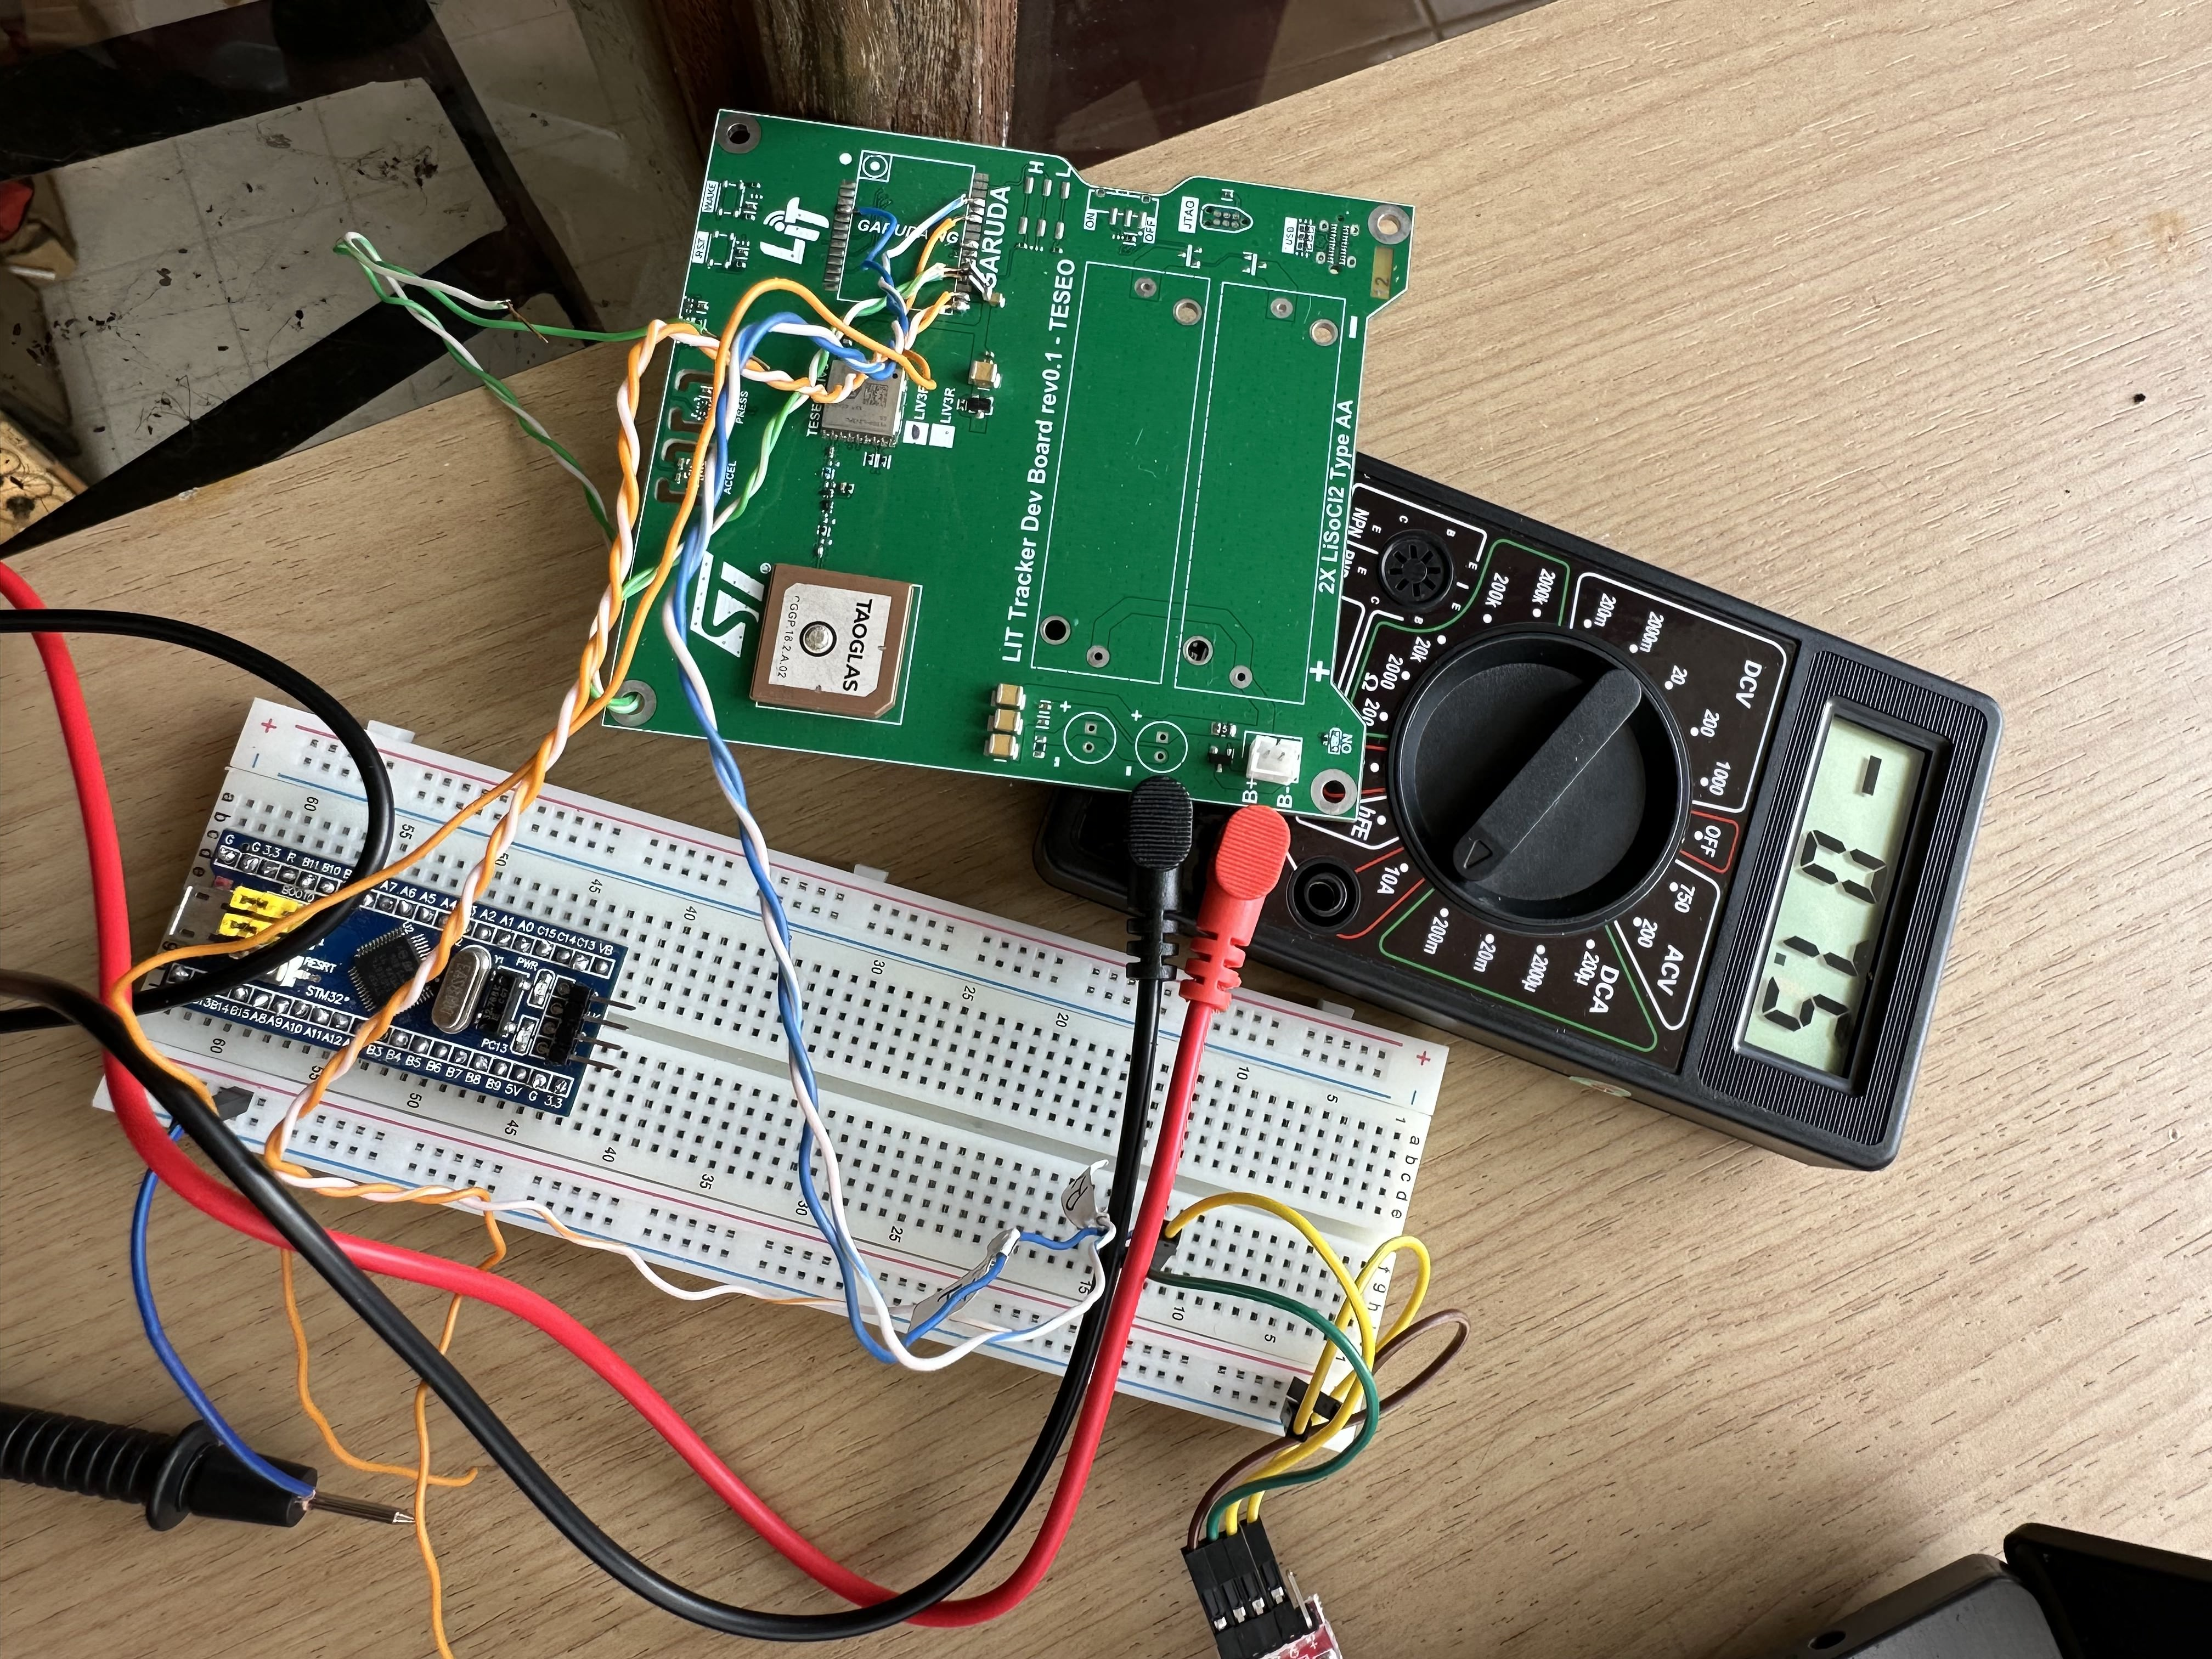
\includegraphics[width=10cm]{contents/chapter-4/low-power.jpg}
	\caption{Modul GNSS yang telah Terangkai dengan Multimeter}
	\label{Fig: low-power-connected}
\end{figure}

Algoritma daya rendah yang digunakan pada pengujian ini adalah mode periodik. Pada mode periodik modul Teseo-LIV3FL akan berada dalam mode akuisisi dalam waktu tertentu hingga mendapat posisi \textit{fix}. Ketika sudah mendapatkan posisis \textit{fix} maka modul Teseo-LIV3FL akan menuju mode \textit{stand by} dan akan menuju dalam mode akuisisi kembali setelah waktu tertentu. Jika modul Teseo-LIV3FL tidak bisa mendapatkan posisi \textit{fix} maka ia juga akan menuju mode \textit{stand by} dan akan mencoba mendapatkan \textit{fix} kembali setelah periode waktu tertentu.

\begin{figure}[H]
	\centering
	\captionsetup{justification=centering}
	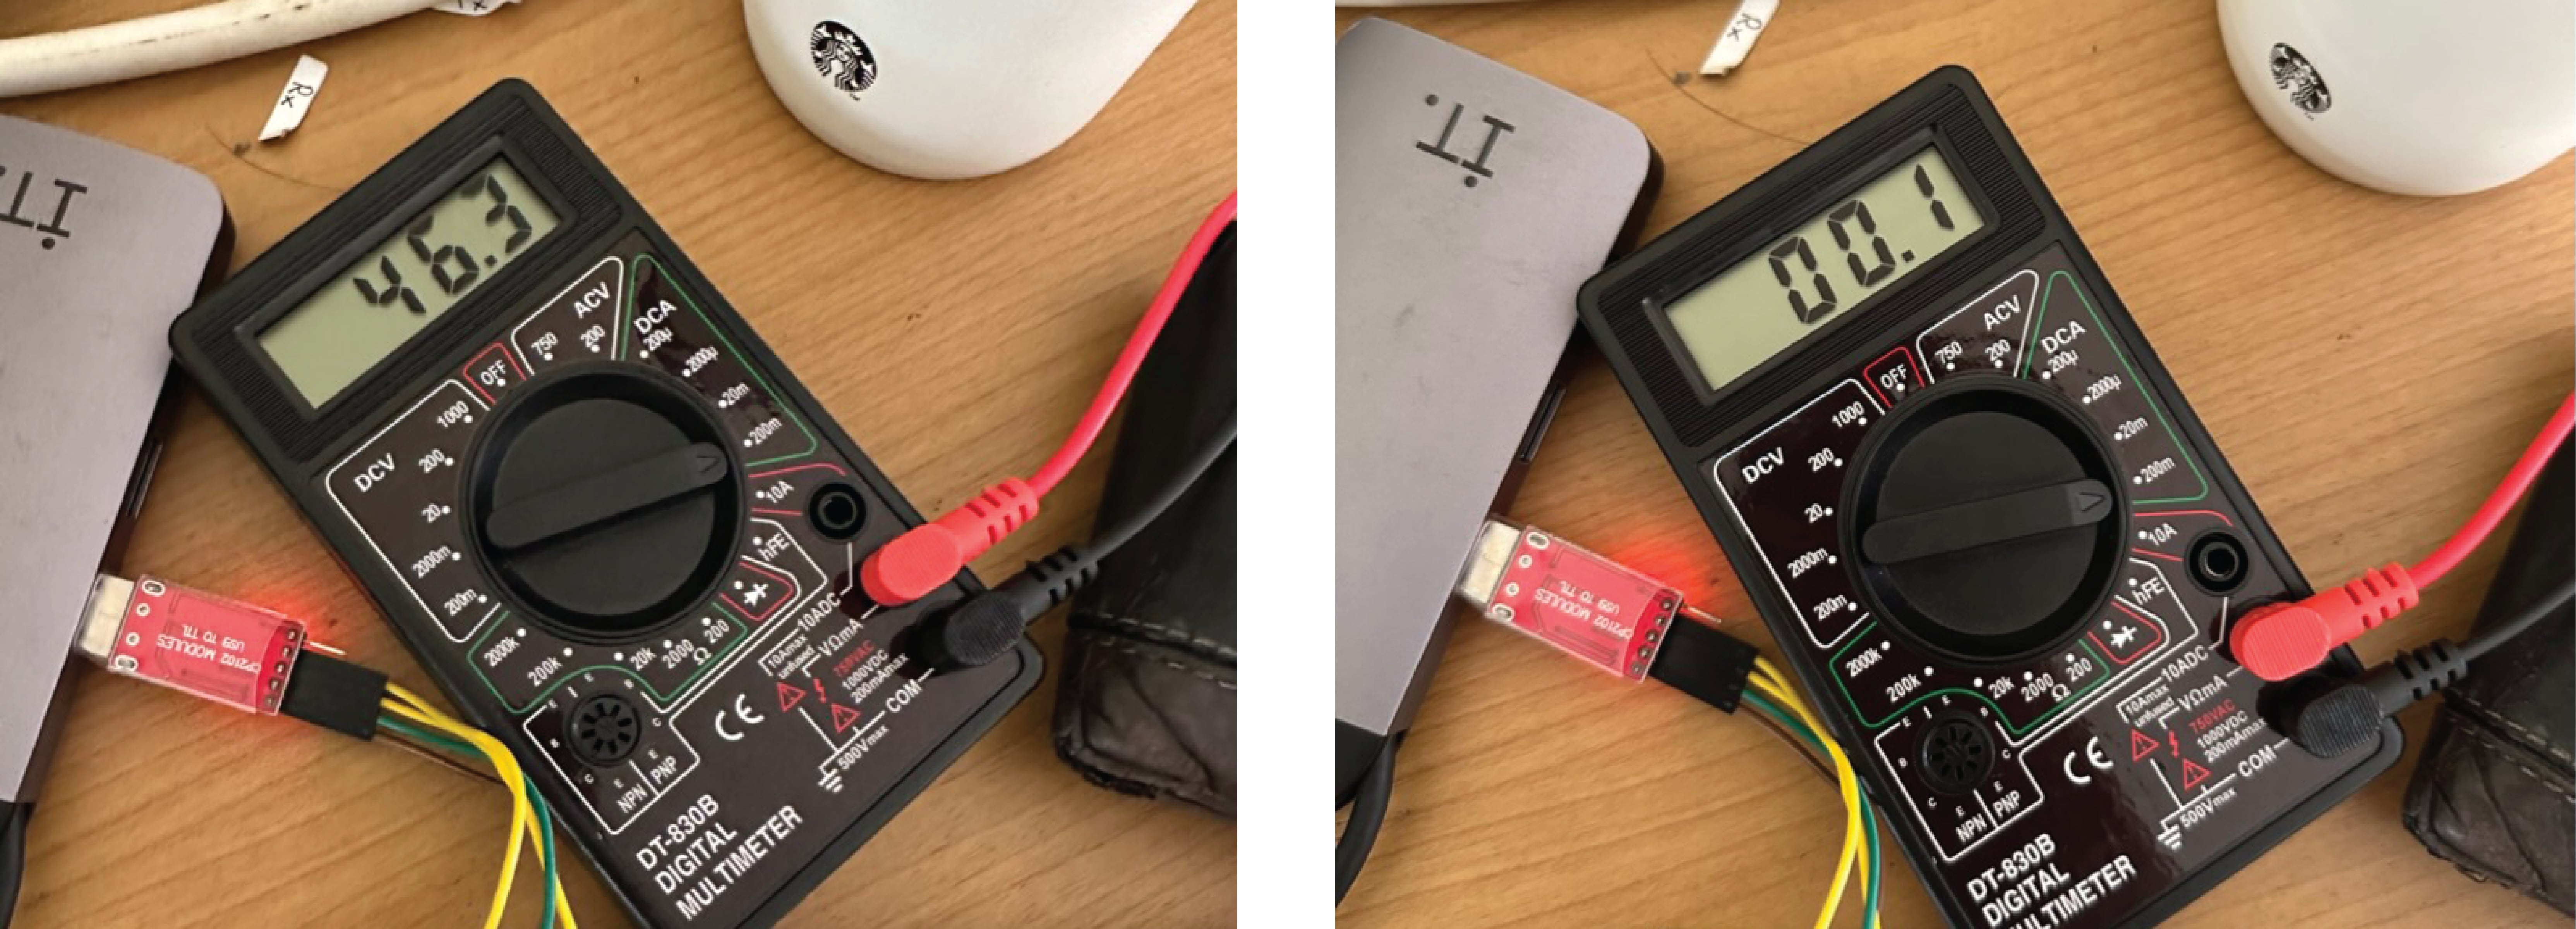
\includegraphics[width=14cm]{contents/chapter-4/low-power-result.jpg}
	\caption{Pembacaan Multimeter pada Mode Akuisisi (Kiri) dan Mode \textit{Stand By} (Kanan)}
	\label{Fig: low-power-result}
\end{figure}

Untuk menyalakan mode daya rendah dapat dilakukan dengan mengirimkan perintah \$PSTMLOWPOWERONOFF. Perintah \$PSTMLOWPOWERONOFF menerima empat belas argumen dengan argumen kedua s.d. kelima untuk mode adaptif, dua argumen selanjutnya untuk mode \textit{cyclic}, dan delapan argumen terakhir untuk mode periodik. Karena digunakan mode periodik maka argumen kedua sampai dengan ketujuh harus diisi dengan angka nol. Perintah yang dikirimkan pada pengujian ini adalah sebagai berikut

\begin{verbatim}
	$PSTMLOWPOWERONOFF,1,0,0,0,0,0,0,3,60,1,1,1,60,30
\end{verbatim}

Perintah di atas akan mengaktifkan mode daya rendah periodik dengan waktu \textit{stand by} selama satu menit setelah mendapatkan tiga posisi \textit{fix}. Selain itu, modul Teseo-LIV3FL akan menuju mode \textit{stand by} selama tiga puluh detik jika tidak dapat mendapatkan posisi \textit{fix} selama satu menit. Detail argumen pada pengujian ini dijelaskan pada Tabel 4.1.

\begin{longtblr}[caption = {Argumen pada Perintah \$PSTMLOWPOWERONOFF}]{
		width = \linewidth,
		colspec = {Q[285]Q[48]Q[608]},
		row{1} = {c},
		row{3} = {c},
		row{5} = {c},
		row{6} = {c},
		row{7} = {c},
		row{8} = {c},
		row{10} = {c},
		row{11} = {c},
		cell{2}{1} = {c},
		cell{2}{2} = {c},
		cell{3}{1} = {c=3}{0.941\linewidth},
		cell{4}{1} = {c},
		cell{4}{2} = {c},
		cell{4}{3} = {r=4}{},
		cell{8}{1} = {c=3}{0.941\linewidth},
		cell{9}{1} = {c},
		cell{9}{2} = {c},
		cell{9}{3} = {r=2}{},
		cell{11}{1} = {c=3}{0.941\linewidth},
		cell{12}{1} = {c},
		cell{12}{2} = {c},
		cell{13}{1} = {c},
		cell{13}{2} = {c},
		cell{14}{1} = {c},
		cell{14}{2} = {c},
		cell{15}{1} = {c},
		cell{15}{2} = {c},
		cell{16}{1} = {c},
		cell{16}{2} = {c},
		cell{17}{1} = {c},
		cell{17}{2} = {c},
		cell{18}{1} = {c},
		cell{18}{2} = {c},
		hline{1-4,8-9,11-12} = {-}{},
	}
	\textbf{Argumen}                               & \textbf{Nilai} & \textbf{Keterangan}                                                                                                                      \\
	Menyalakan atau mematikan mode daya rendah     & 1              & Mode daya rendah dinyalakan                                                                                                              \\
	Mode Adaptif                                   &               0 &                                                                                                                                          \\
	\textit{Constellation mask}                    & 0              & Mode adaptif tidak digunakan.                                                                                                            \\
	Batas EHPE                            &               0 &                                                                                                                                          \\
	Satelit maksimum                               &               0 &                                                                                                                                          \\
	Perpindahan konstelasi otomatis                &         0       &                                                                                                                                          \\
	Mode \textit{cyclic}                           &           0     &                                                                                                                                          \\
	Menyalakan atau mematikan \textit{duty cycle} & 0              & Mode \textit{cyclic} tidak digunakan.\\
	Periode \textit{duty cycle}                    &         0       &                                                                                                                                          \\
	Mode periodik                                  &                &                                                                                                                                          \\
	Mode periodik                                  & 3              & Mode periodik \textit{stand by}                                                                                                          \\
	FixPeriod                                      & 60             & Modul akan memasuki mode~\textit{stand by} selama enam puluh detik setelah mendapat posisi \textit{fix}                                \\
	FixOnTime                                      & 3              & Memasuki mode \textit{stand by~setelah mendapatkan tiga posisi \textit{fix}}                                                             \\
	Penyegaran ephemeris                           & 1              & Penyegaran ephemeris diaktifkan                                                                                                          \\
	Kalibrasi RTC                                  & 1              & Kalibrasi RTC diaktifkan                                                                                                                 \\
	NoFixCnt                                       & 60             & Modul akan memasuki mode \textit{stand by} jika tidak bisa mendapatkan posisi \textit{fix~setelah enam puluh detik (\textit{fix loss)}} \\
	NoFixOff                                       & 30             & Modul memasuki \textit{stand by} selama tiga puluh detik setelah \textit{fix loss}\\
	\hline                                                      
\end{longtblr}

Dalam mode akuisisi, arus yang mengalir pada modul Teseo-LIV3FL adalah sebesar 46.3 mA atau  18,7 mA lebih kecil jika dibandingkan dengan \textit{datasheet}. Pada mode \textit{stand by}, arus yang mengalir pada modul Teseo-LIV3FL sudah mendekati \textit{datasheet} (10$\mu$A), yaitu sebesar 15 $\mu$A. Gambar \ref{Fig: low-power-result} sebelah kiri menunjukan hasil pengukuran multimeter ketika modul Teseo-LIV3FL berada dalam mode akuisisi dan sebelah kanan ketika modul Teseo-LIV3FL berada dalam mode \textit{stand by}.

\section{Pengujian \textit{Rapid Static Survey}}
Rapid Static Survey adalah pengujian yang dilakukan untuk meninjau performa modul GNSS dalam keadaan diam. Pengujian ini dapat dilakukan dalam rentang waktu lima belas menit s.d. dua jam (Lauer, 2018). Pengujian ini akan meninjau  dan presisi dari modul GNSS. Akurasi adalah tingkat kedekatan hasil pembacaan modul GNSS dengan posisi sebenarnya, sedangkan tingkat presisi menunjukan seberapa dekat hasil yang didapat dengan rata-rata dari seluruh sampel (Novatel, 2003).

Pada pengujian rapid static survey, modul Teseo-LIV3FL diletakan dalam empat skenario selama satu jam. Skenario tersebut meliputi \textit{basemet}, dalam ruangan, ruangan semi terbuka, dan ruang terbuka. Pengujian setiap skenario dilakukan pada empat titik di lingkungan Universitas Gadjah Mada, yaitu:
\begin{enumerate}
	\item \textit{Basement} diwakili oleh tempat parkir bawah tanah milik Fakultas Ilmu Sosial dan Ilmu Politik.
	\item Ruangan tertutup diwakili oleh Lantai 5 Gedung SGLC Fakultas Teknik
	\item Ruang semi terbuka diwakili oleh Selasar Grha Sabha Pramana.
	\item Ruangan terbuka diwakili oleh Lapangan Pancasila
\end{enumerate}

Modul Teseo-LIV3FL dihubungkan dengan protokol komunikasi UART pada baud rate 115.200 Bps menggunakan konversi USB to TTL. Pengujian ini akan meninjau nilai HDOP, VDOP, PDOP, dan CEP di setiap skenario.

\subsection{Skenario \textit{Basement}}
\begin{table}[H]
	\caption{Hasil Pengujian Skenario \textit{Basement}}
	\vspace{0.5em}
	\centering
	\begin{tabular}{ccccc}
		\hline
		& \textbf{Minima} & \textbf{Maxima} & \textbf{Rata-rata} & \textbf{Standar Deviasi}\\
		\hline 
		HDOP & 1,80 & 26,80 & 8,27 & 5,36\\
		PDOP & 2,80 & 39,30 & 10,67 & 7,30\\
		VDOP & 2,00 & 28,80 & 8,27 & 5,36\\
		CEP (m) & 0 & 79,56 & 32,69 & 13,34\\
		Jumlah Satelit & 5 & 12 & 7,60 & 1,27\\
		\hline
	\end{tabular}
	\label{Tab: basement-table}
\end{table}

Pengujian skenario \textit{basement} dilakukan untuk mengetahui performa modul Teseo-LIV3FL pada ruangan bawah tanah. Modul Teseo-LIV3FL diletakan di tempat parkir bawah tanah milik Fakultas Ilmu Sosial dan Ilmu Politik. Lingkungan pengujian berada di bawah gedung empat lantai dengan struktur beton. Selain itu, terdapat sedikit bagian terbuka yang memungkinkan sinar matahari untuk memasuki ruangan. Gambar \ref{Fig: basement-keadaan} menunjukan kondisi pengujian skenario \textit{basement}.

\begin{figure}[H]
	\centering
	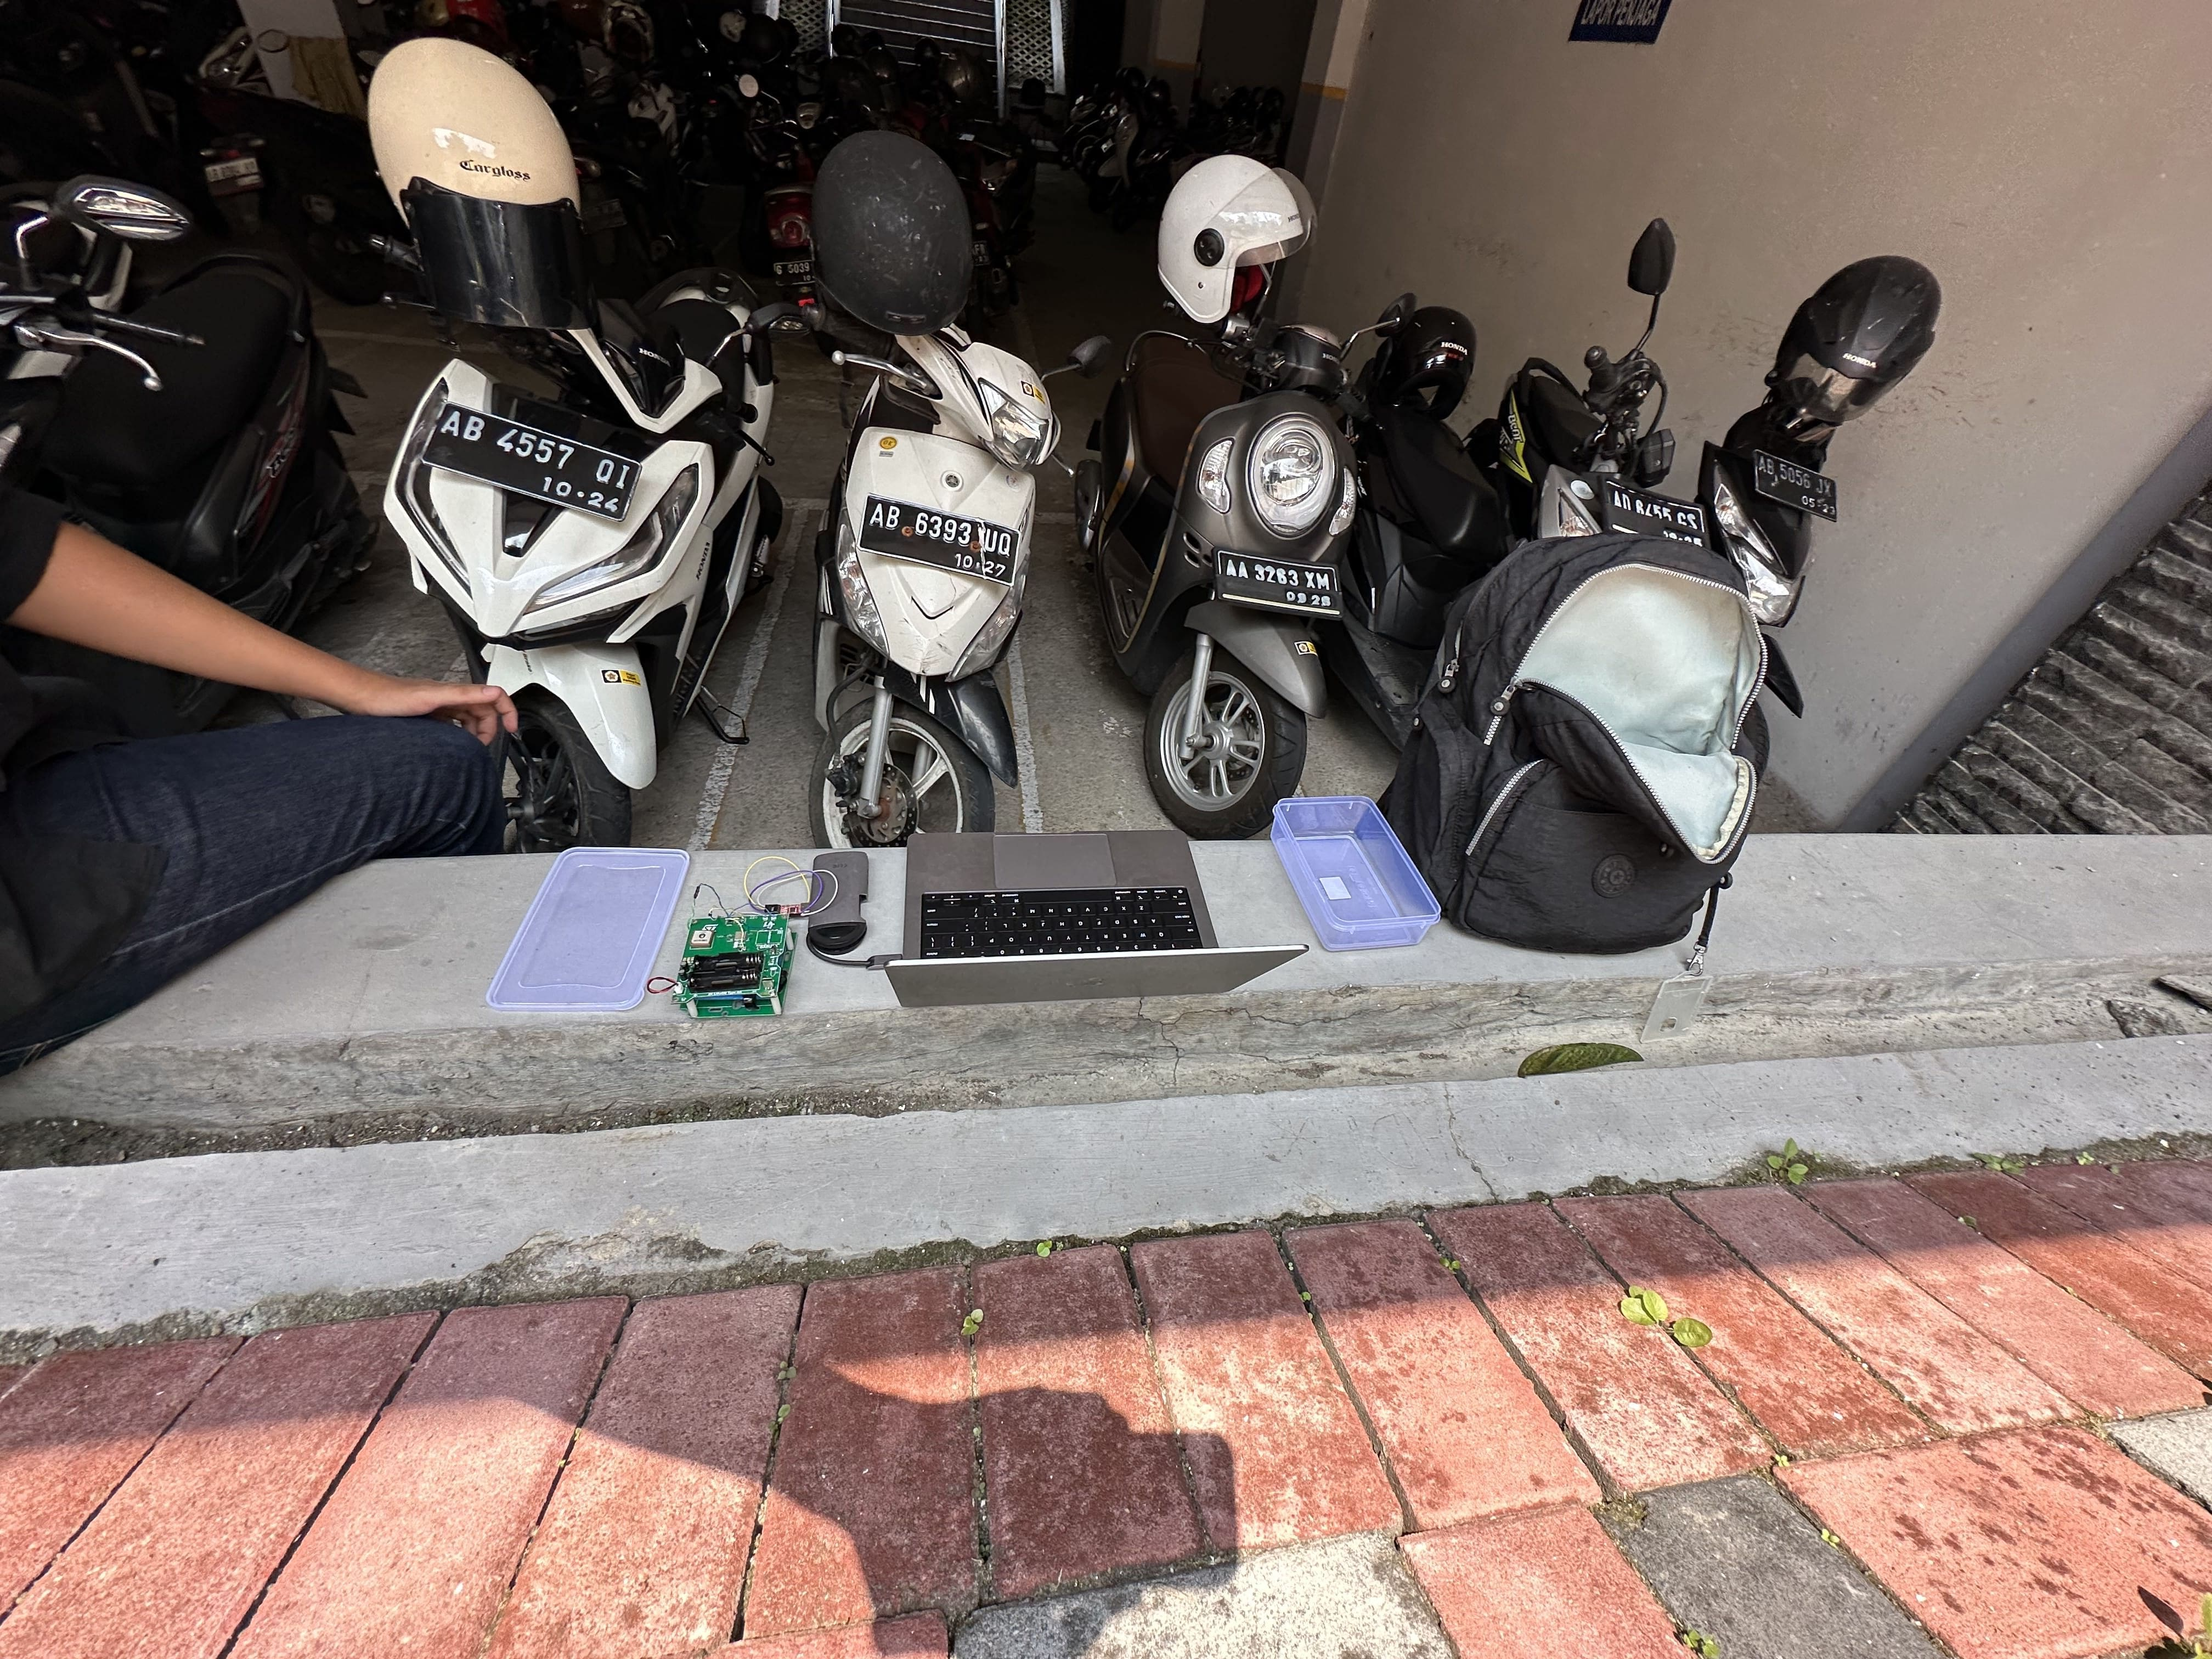
\includegraphics[width=10cm]{contents/chapter-4/1-skenario-basement/keadaan.jpg}
	\caption{Pengujian Skenario \textit{Basement}}
	\label{Fig: basement-keadaan}
\end{figure}

Hasil pembacaan modul Teseo-LIV3FL pada skenario \textit{basement} tidak memberikan hasil yang akurat. Terlihat pada Gambar \ref{Fig: basement-sats_dop} bahwa terjadi lonjakan nilai DOP. Tabel \ref{Tab: basement-table} menunjukan nilai maksimum DOP adalah nilai PDOP sebesar 39,30. Nilai PDOP yang sangat tinggi menunjukan bahwa persebaran satelit di langit tidak mencakup seluruh lingkaran seperti ditunjukan oleh \textit{sky plot} pada Gambar \ref{Fig: basement-skyplot}. \textit{Sky plot} tersebut menunjukan bahwa persebaran satelit hanya mencakup setengah bagian pada lingkaran.

\begin{figure}[H]
	\centering
	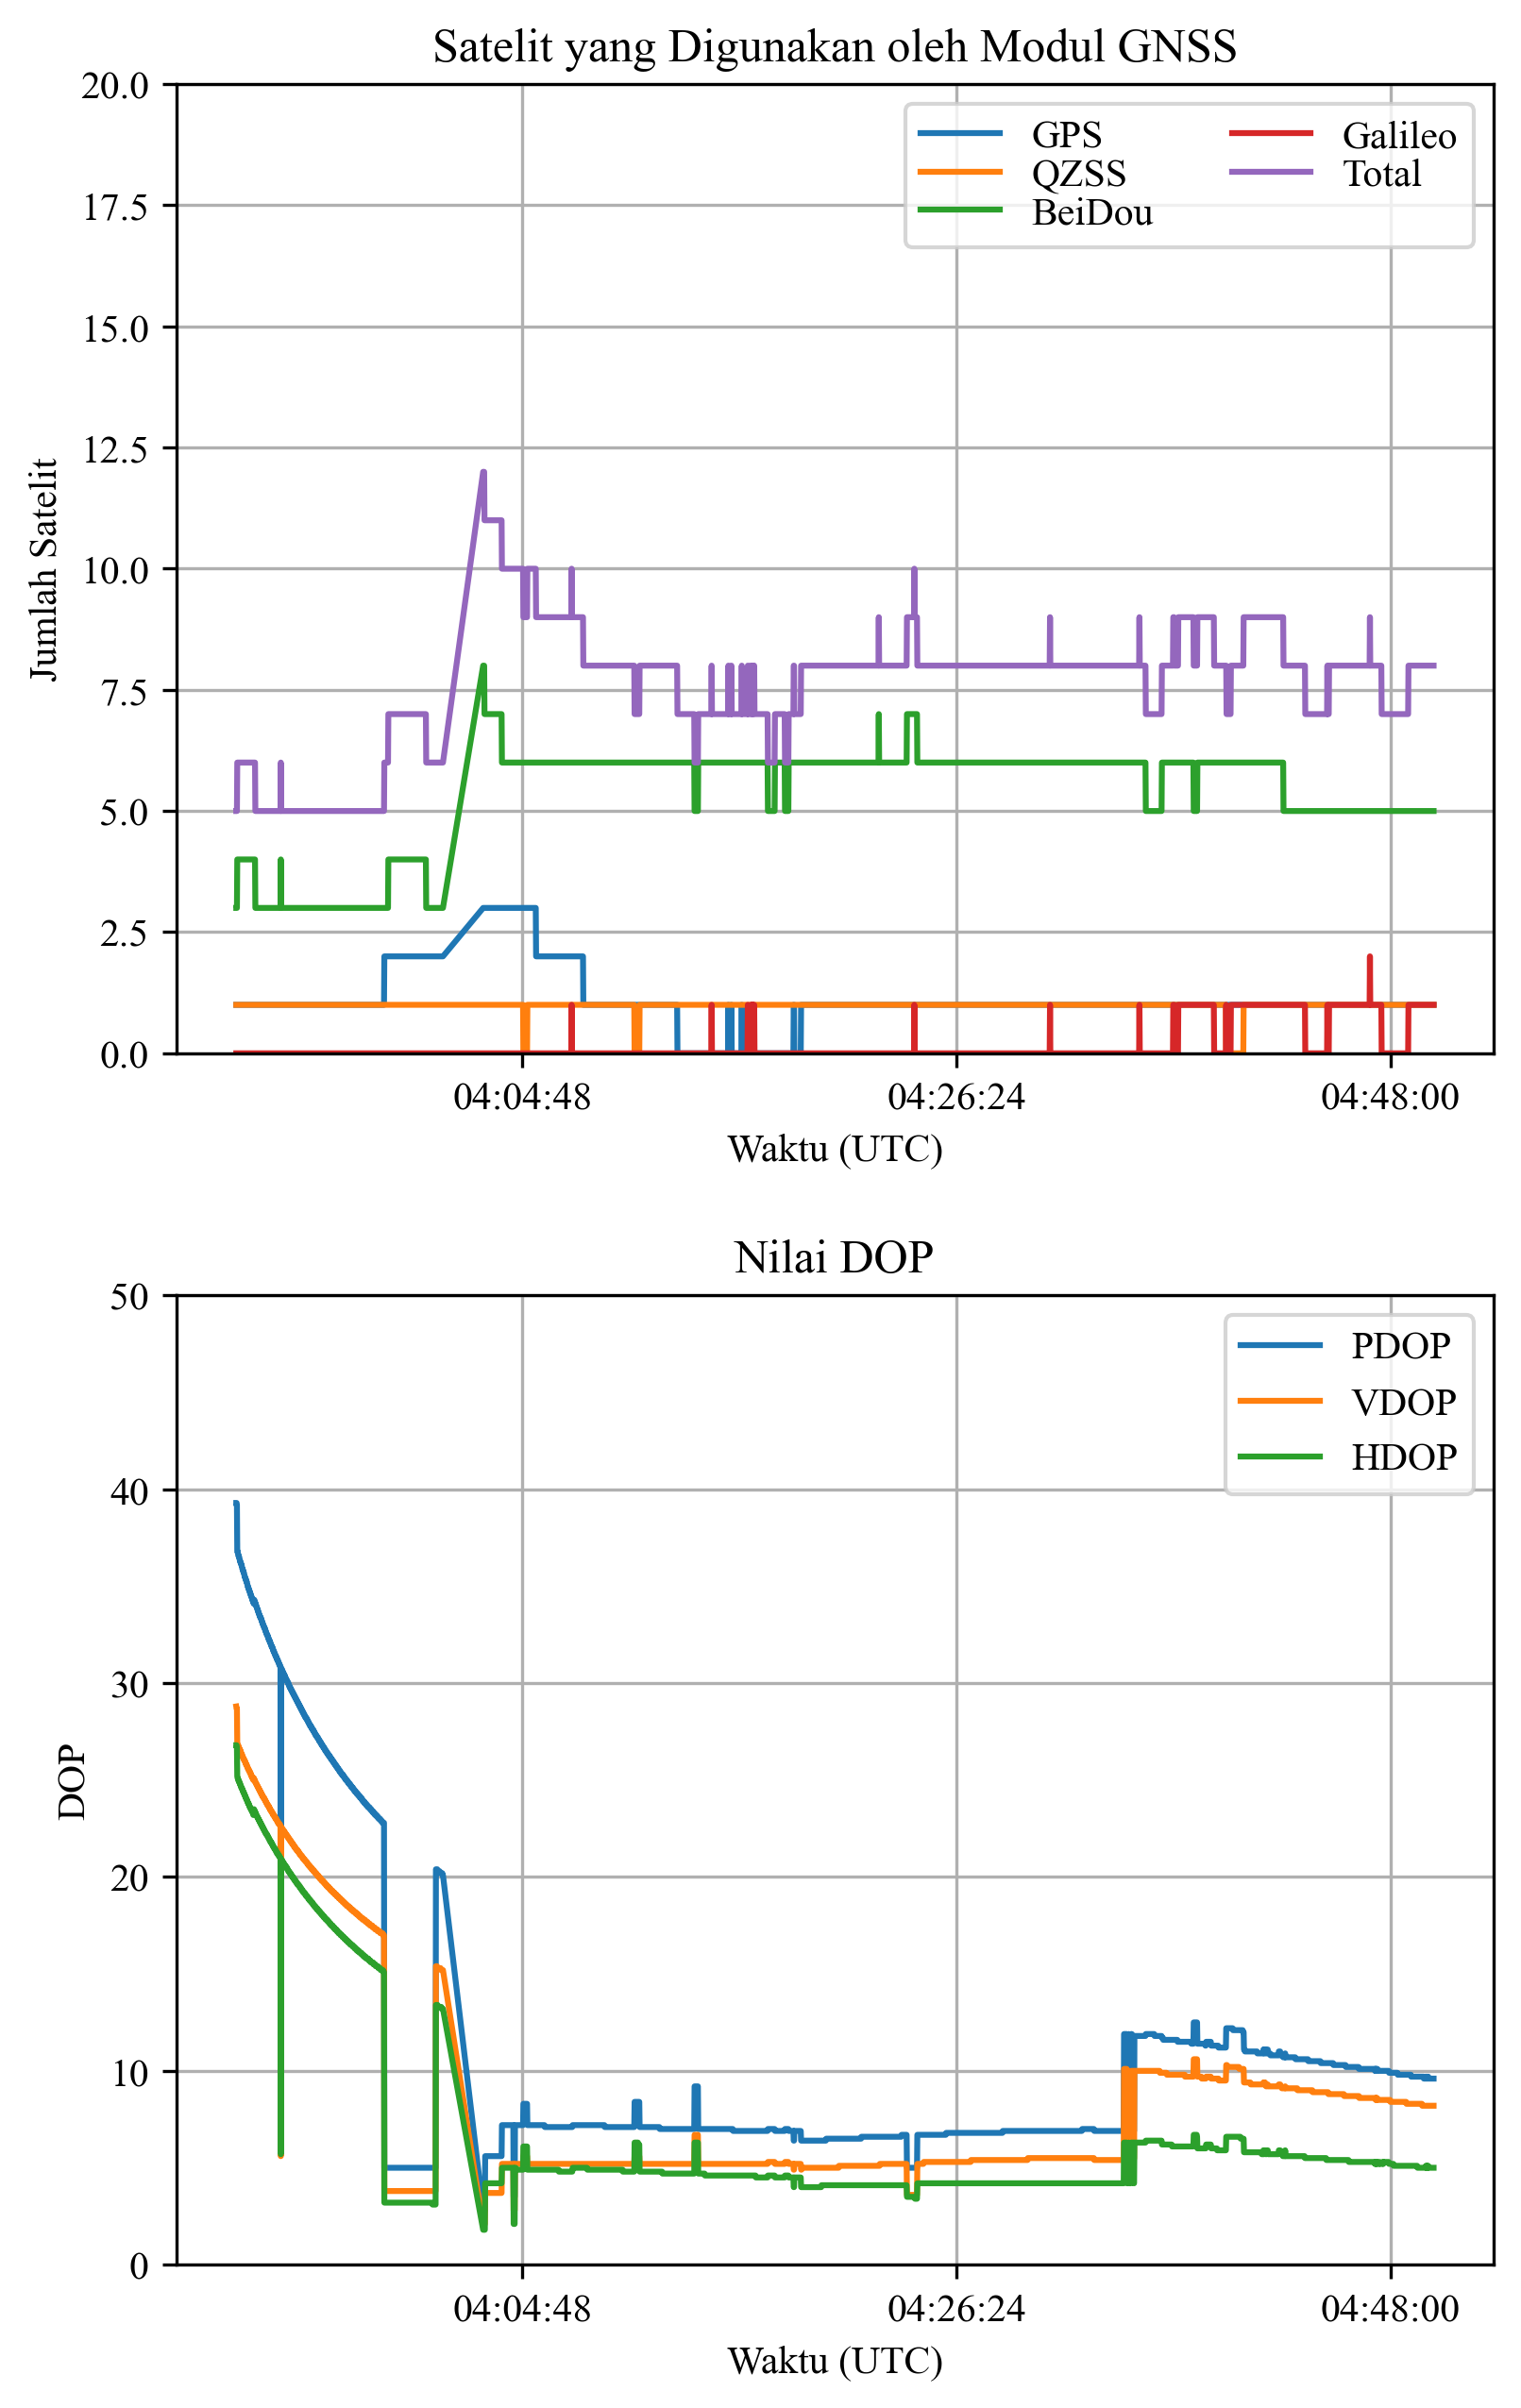
\includegraphics[width=12cm]{contents/chapter-4/1-skenario-basement/sats_dop.png}
	\caption{DOP dan Visibilitas Satelit Pengujian Skenario \textit{Basement}}
	\label{Fig: basement-sats_dop}
\end{figure}

Pada skenario \textit{basement}, modul Teseo-LIV3FL tetap dapat menangkap isyarat dari keempat konstelasi Teseo-LIV3FL yang telah diatur meskipun tertutup oleh struktur beton. Konstelasi dengan jumlah satelit adalah BeiDou milik Republik Rakyat Tiongkok. Lonjakan nilai DOP pada awal pengujian terjadi bersamaan dengan keadaan jumlah satelit paling rendah. Hal tersebut menunjukan bahwa jumlah satelit yang rendah akan meningkatkan ketiga nilai DOP yang artinya akan menurunkan akurasi dari hasil pembacaan modul Teseo-LIV3FL.

\begin{figure}[H]
	\centering
	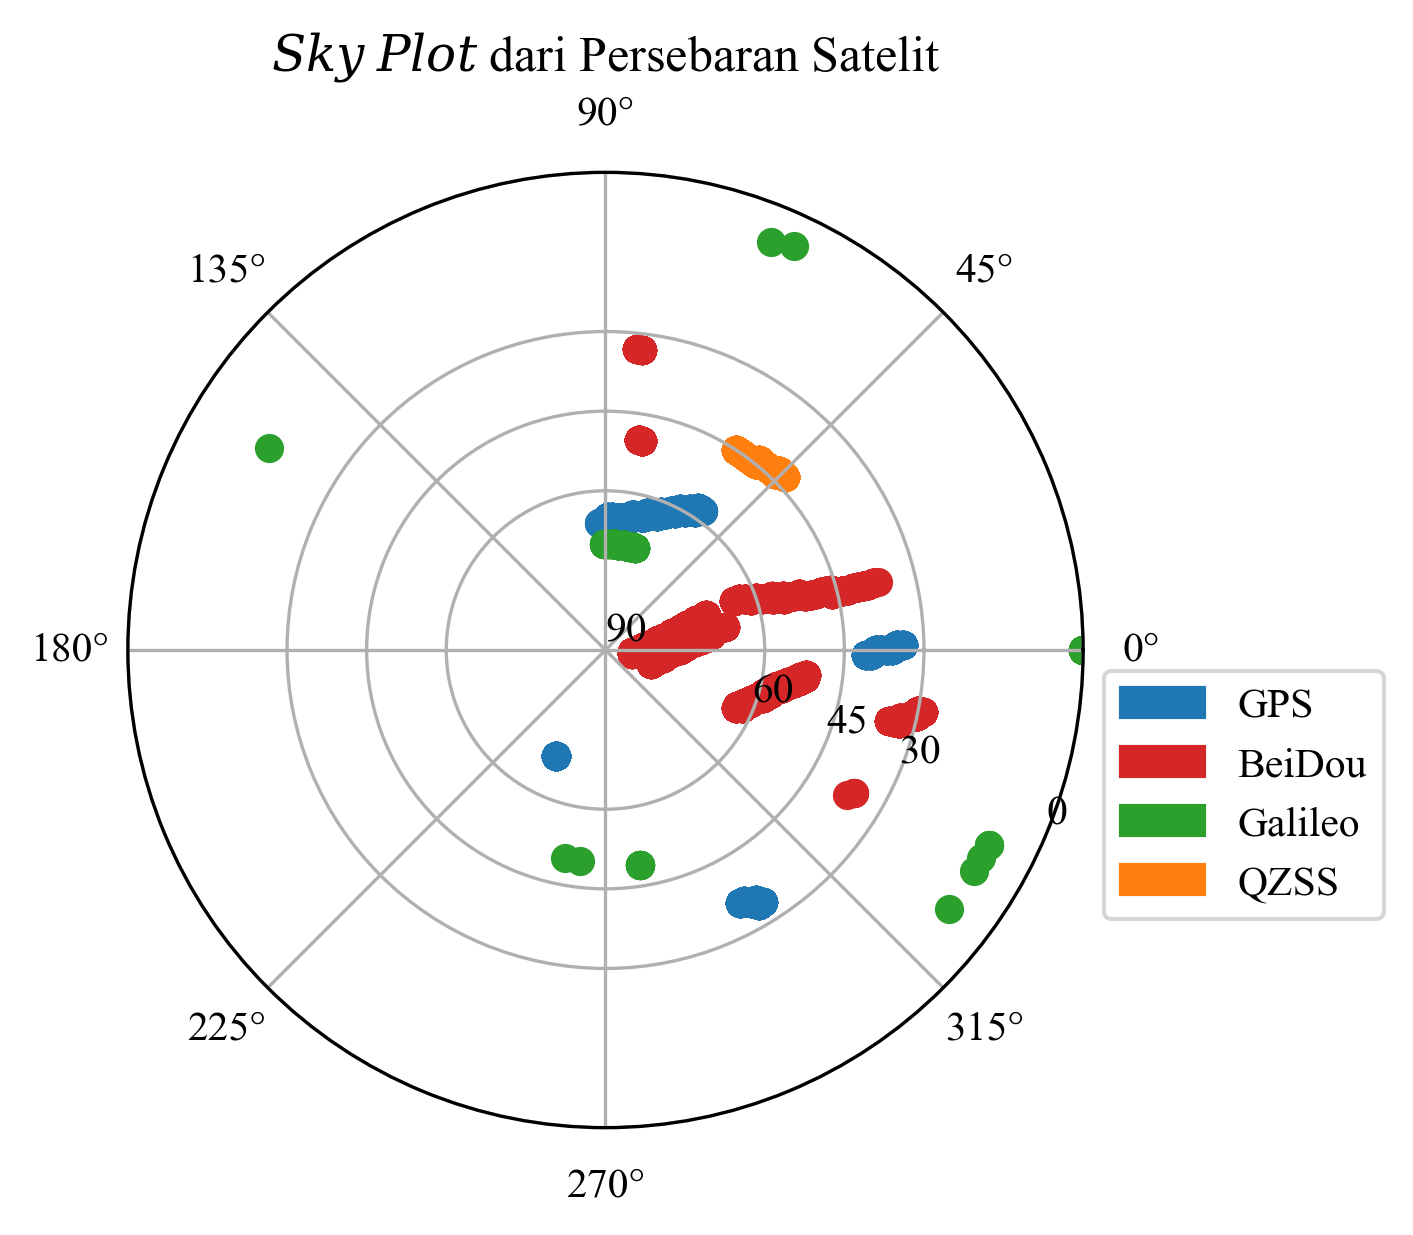
\includegraphics[width=11cm]{contents/chapter-4/1-skenario-basement/skyplot.png}
	\caption{\textit{Sky Plot} Pengujian Skenario \textit{Basement}}
	\label{Fig: basement-skyplot}
\end{figure}

Nilai rata-rata nilai CEP pada pengujian ini adalah 32,69 m yang menunjukan tingkat presisi pada skenario \textit{basement} adalah 32,69 m. Selain itu, rata-rata nilai HDOP pada skenario \textit{basement} menunjukan angka 8,27 yang menunjukan bahwa hasil pengukuran posisi pada skenario ini masih layak untuk digunakan.

Pengujian skenario \textit{basement} menunjukan bahwa modul GNSS masih bisa digunakan dalam ruangan bawah tanah dengan sedikit bagian terbuka. Meskipun mampu untuk mendapatkan posisi \textit{fix}, akurasi yang didapat masih bisa diperbaiki pada skenario selanjutnya.

\subsection{Skenario Dalam Ruangan}
\begin{table}[H]
	\caption{Hasil Pengujian Dalam Ruangan}
	\vspace{0.5em}
	\centering
	\begin{tabular}{ccccc}
		\hline
		& \textbf{Minima} & \textbf{Maxima} & \textbf{Rata-rata} & \textbf{Standar Deviasi}\\
		\hline 
		HDOP & 1,30 & 6,80 & 2,79 & 0,68\\
		PDOP & 2,00 & 8,40 & 3,73 & 0,74\\
		VDOP & 1,40 & 5,50 & 2,48 & 0,94\\
		CEP (m) & 9,51	& 33,27 & 12,14 & 4,02\\
		Jumlah Satelit & 8 & 15 & 10,93 & 1,14\\
		\hline
	\end{tabular}
	\label{Tab: indoor-table}
\end{table}

Pengujian skenario dalam ruangan dilakukan untuk meninjau performa modul Teseo-LIV3FL di dalam ruangan tertutup. Titik pengujian berada di lantai 5 Gedung SGLC Fakultas Teknik. Lingkungan sekitar pengujian merupakan suatu ruangan dengan jendela besar yang memungkinkan lebih banyak sinar matahari untuk memasuki ruangan. Gambar \ref{Fig: indoor-keadaan} menunjukan pengujian skenario dalam ruangan.

\begin{figure}[ht]
	\centering
	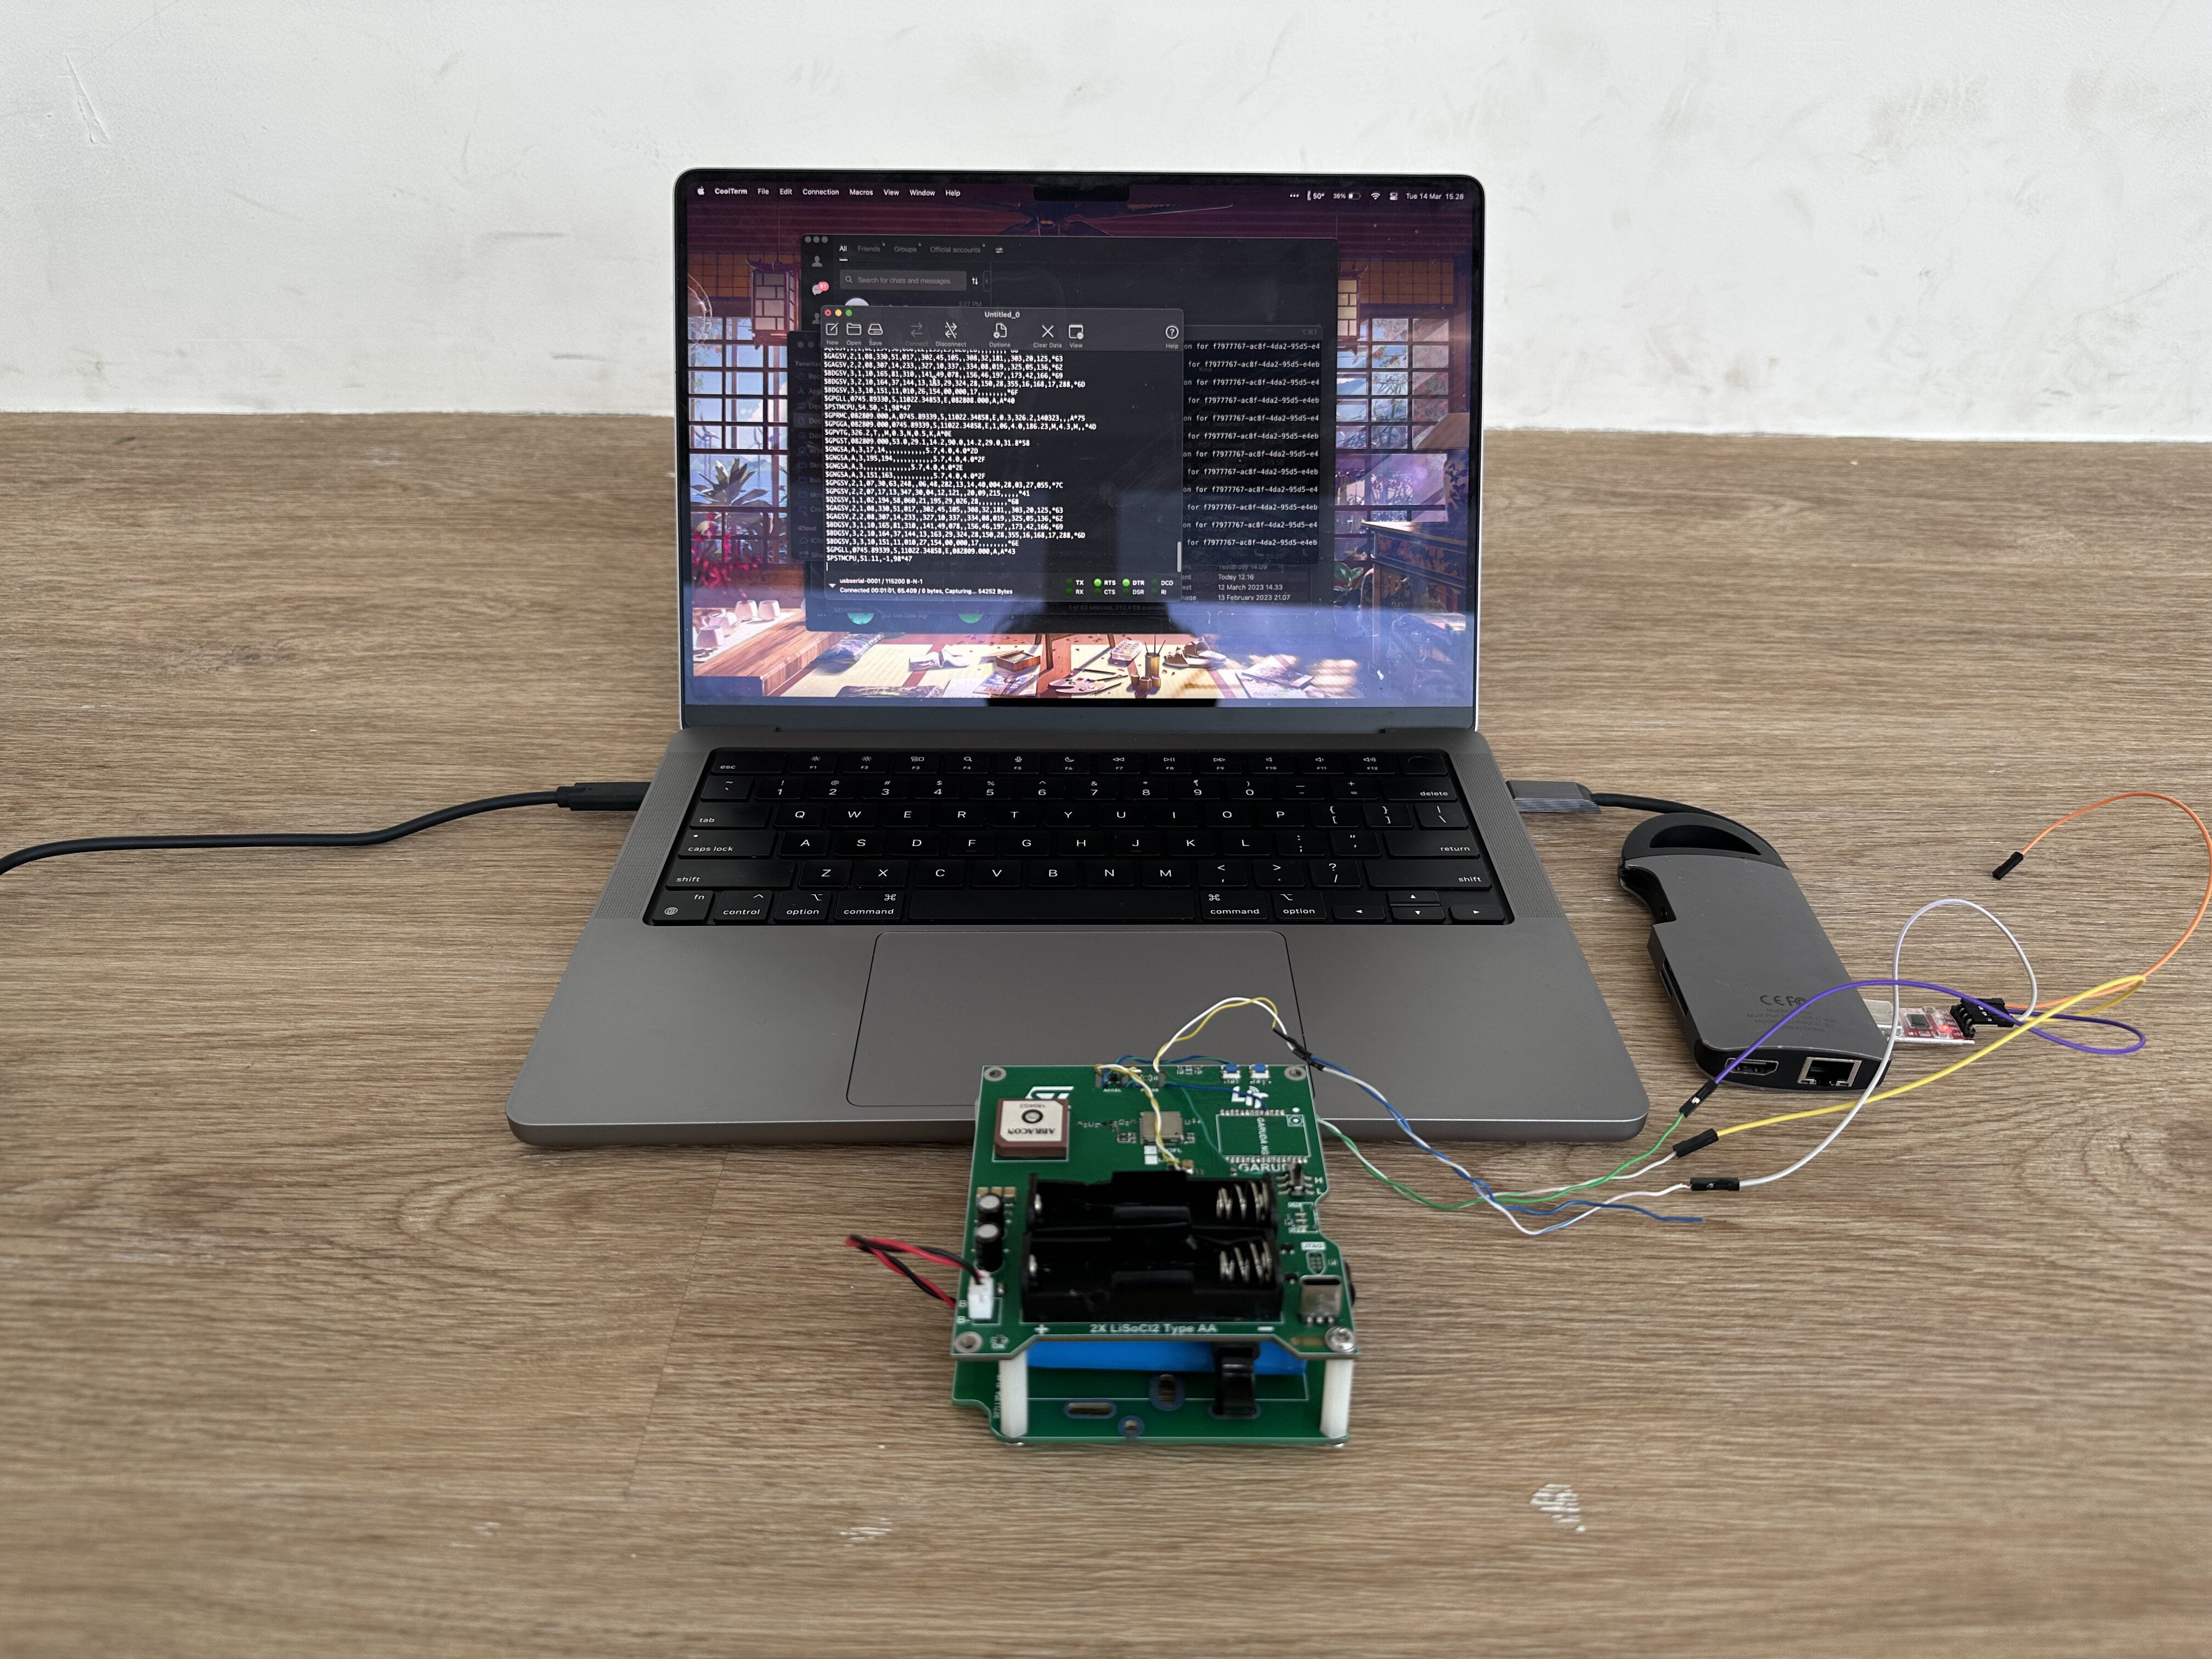
\includegraphics[width=10cm]{contents/chapter-4/2-skenario-indoor/keadaan.jpg}
	\caption{Pengujian Skenario Dalam Ruangan}
	\label{Fig: indoor-keadaan}
\end{figure}

Sama seperti pada pengujian skenario \textit{basement}, modul Teseo-LIV3FL juga dapat menerima isyarat dari keempat konstelasi yang telah diatur sebelumnya seperti ditunjukan pada Gambar \ref{Fig: indoor-sats_dop}. Konstelasi dengan jumlah satelit paling banyak adalah BeiDou dan GPSS. Jumlah satelit pada konstelasi QZSS hampir selalu konstan pada sebanyak dua buah, sedangkan konstelasi Galileo bervariasi antara nol s.d. empat buah satelit.

\begin{figure}[H]
	\centering
	\captionsetup{justification=centering}
	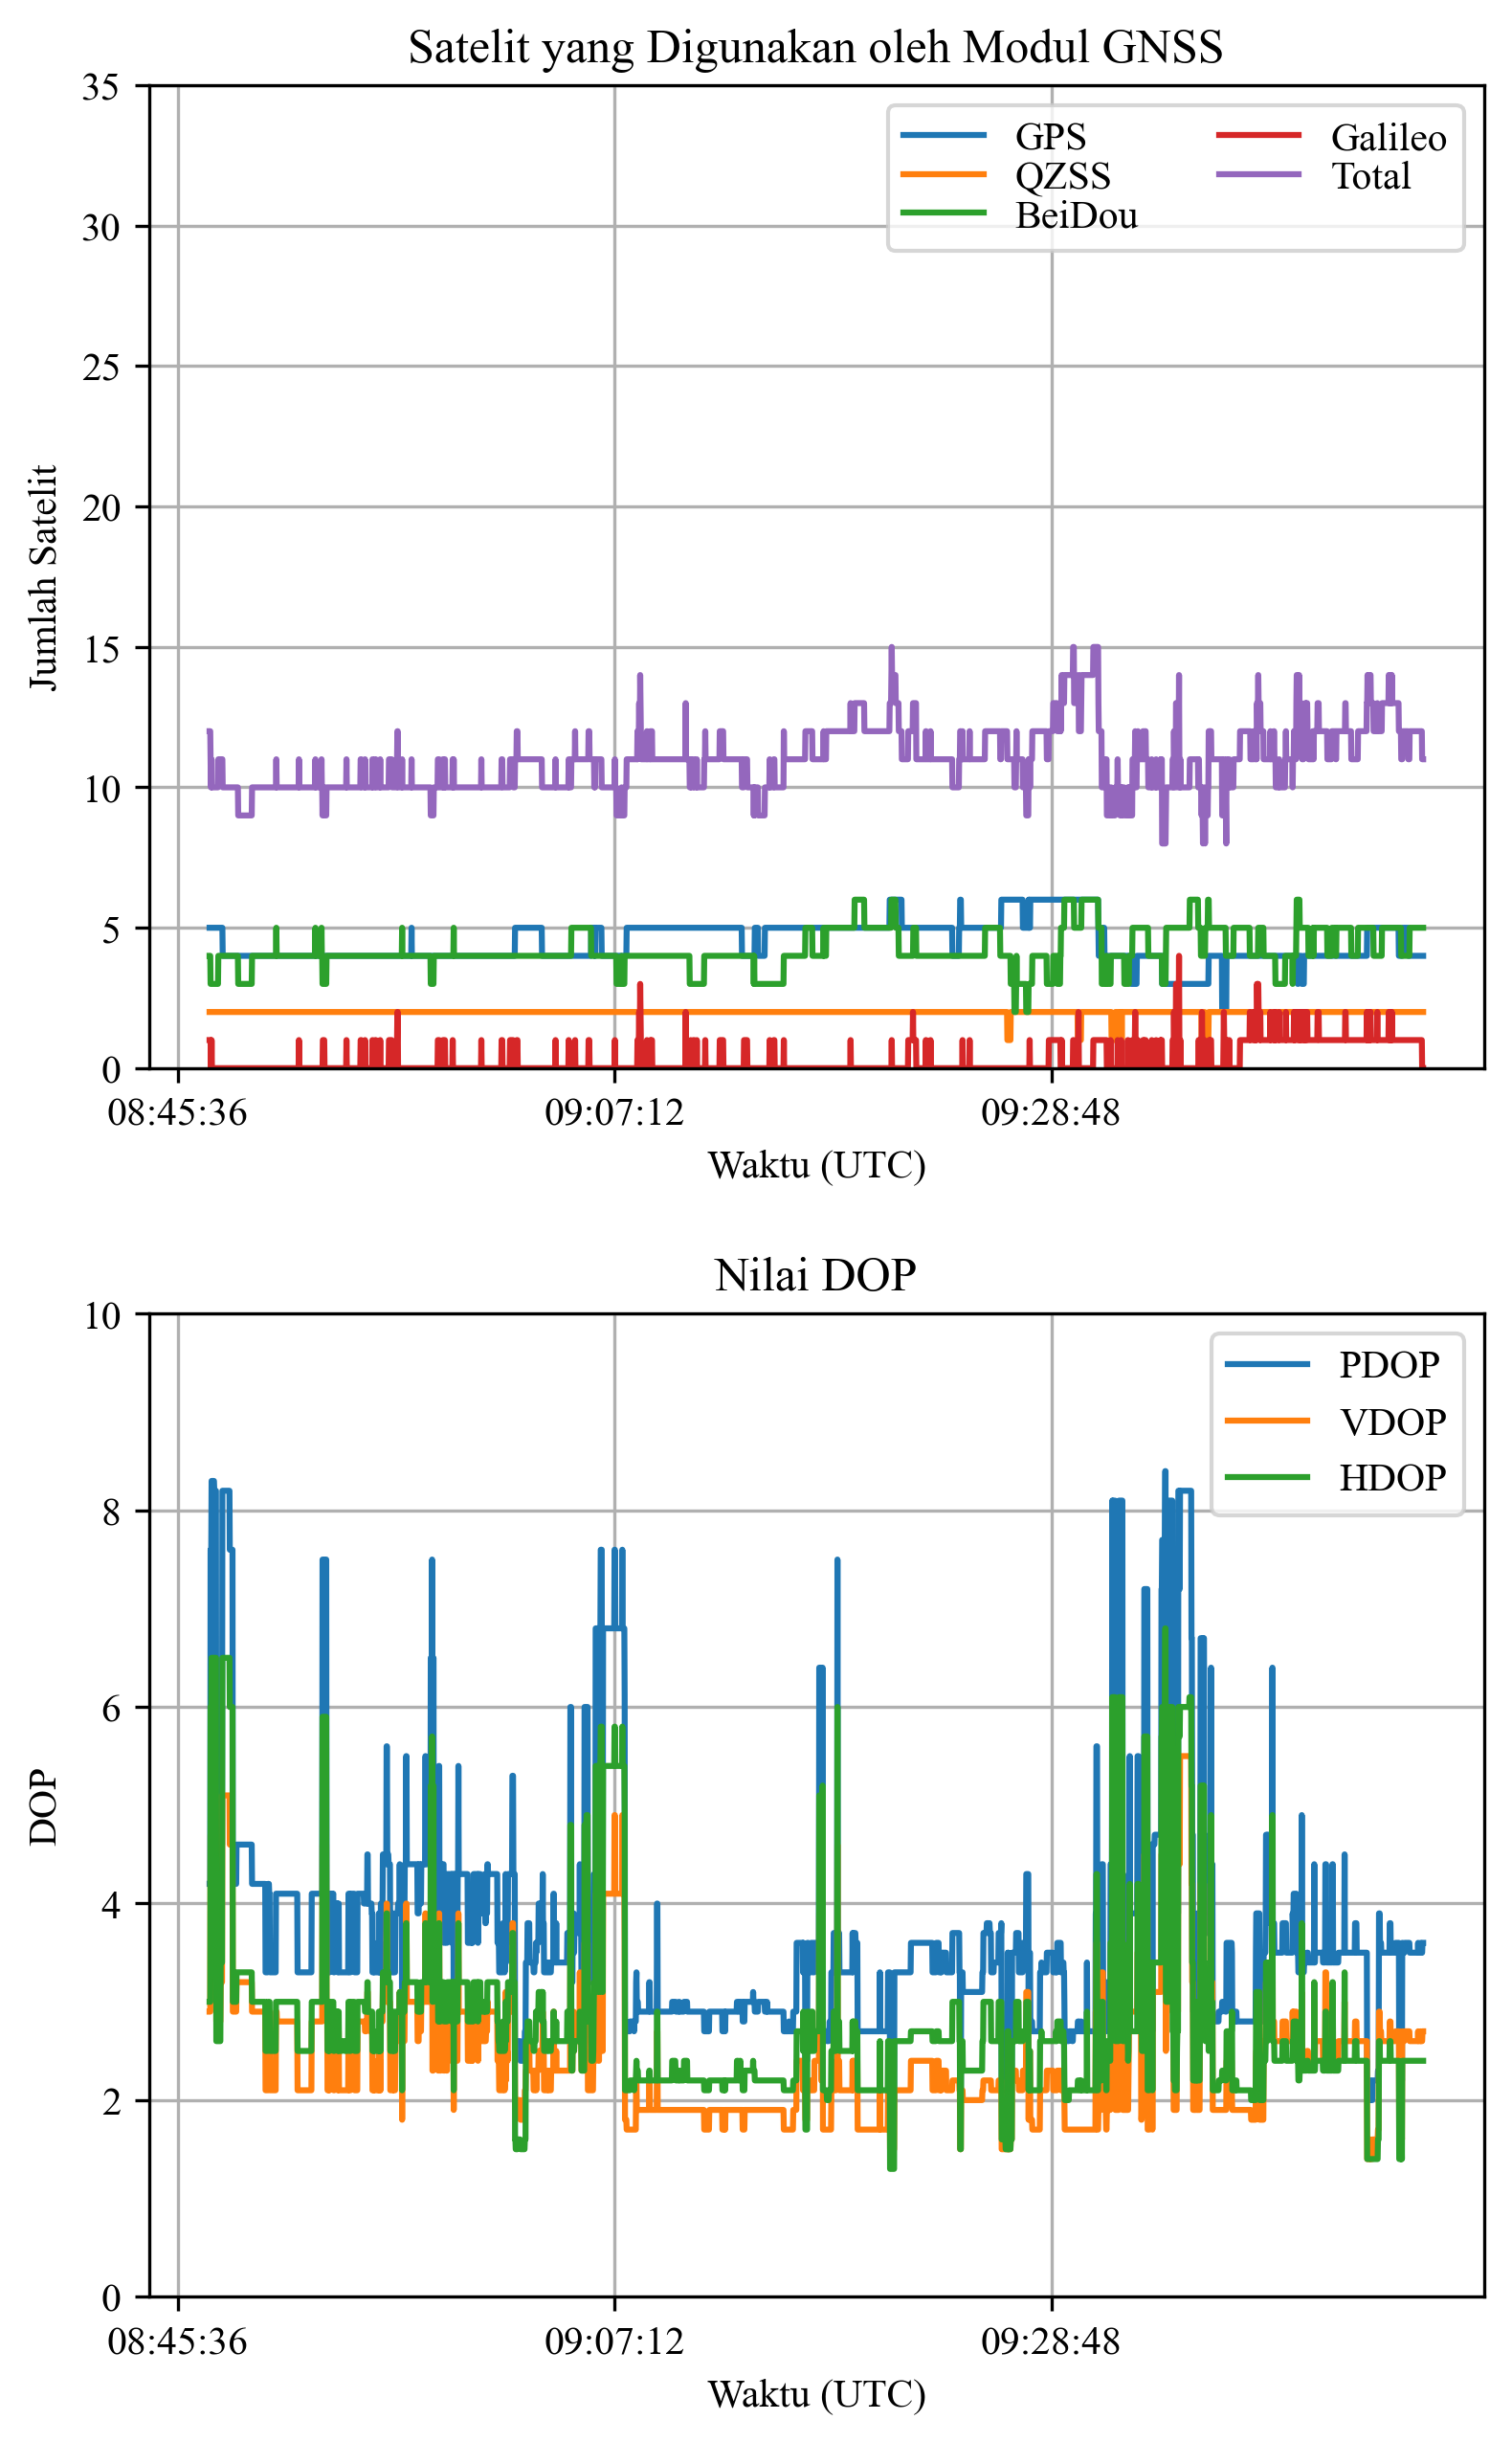
\includegraphics[width=12cm]{contents/chapter-4/2-skenario-indoor/sats_dop.png}
	\caption{DOP dan Visibilitas Satelit Pengujian Skenario Dalam Ruangan Tertutup}
	\label{Fig: indoor-sats_dop}
\end{figure}

Nilai DOP yang lebih rendah menunjukan bahwa akurasi pada skenario ini lebih baik jika dibandingkan dengan skenario sebelumnya. Rata-rata nilai PDOP pada skenario ini adalah 3,73. Hal tersebut juga bersamaan dengan cakupan satelit yang lebih memenuhi lingkaran seperti ditunjukan oleh Gambar \ref{Fig: indoor-sky_plot}.

\begin{figure}[H]
	\centering
	\captionsetup{justification=centering}
	\includegraphics[width=12cm]{contents/chapter-4/2-skenario-indoor/sky_plot.png}
	\caption{\textit{Sky Plot} Skenario Dalam Ruangan}
	\label{Fig: indoor-sky_plot}
\end{figure}

Rata-rata CEP pada skenario dalam ruangan adalah 12,14 m atau 37,14\% lebih presisi jika dibandingkan dengan skenario \textit{basement}. Tabel \ref{Tab: indoor-table} menunjukan bahwa rata-rata nilai HDOP pada pengujian ini adalah 2,79 yang menunjukan bahwa hasil pengukuran sudah baik dan tepat berada pada standar minimum pengukuran. Struktur beton yang lebih sedikit dapat membantu untuk meningkatkan performa GNSS terlihat pada semakin banyak satelit yang dapat digunakan dan penurunan pada nilai CEP dan ketiga nilai DOP.

\subsection{Skenario Ruangan Semi Terbuka}
\begin{table}[H]
	\caption{Hasil Pengujian di Ruangan Semi Terbuka}
	\vspace{0.5em}
	\centering
	\begin{tabular}{ccccc}
		\hline
		& \textbf{Minima} & \textbf{Maxima} & \textbf{Rata-rata} & \textbf{Standar Deviasi}\\
		\hline 
		HDOP & 0,80 & 1,40 & 0,91 & 0,12\\
		PDOP & 1,50	& 3,00 & 1,75 & 0,25\\
		VDOP & 1,20	& 2,70 & 1,49 & 0,23\\
		CEP (m) & 7,28	& 28,32 & 13,83 & 5,49\\
		Jumlah Satelit & 10 & 18 & 14,32 & 1,41\\
		\hline
	\end{tabular}
	\label{Tab: semioutdoor-table}
\end{table}

Pengujian skenario ruangan semi terbuka bertujuan untuk meninjau performa modul Teseo-LIV3FL di luar ruangan dengan penghalang seperti pohon, atap, dan lain-lain. Titik pengujian berada di Selasar Grha Sabha Pramana. Lingkungan sekitar pengujian berupa ruangan semi terbuka dengan penghalang berupa tingkat dua Grha Sabha Pramana dan pepohonan di sekitar ruangan. Gambar \ref{Fig: semioutdoor-keadaan} menunjukan pengujian skenario ruangan semi terbuka.

\begin{figure}[H]
	\centering
	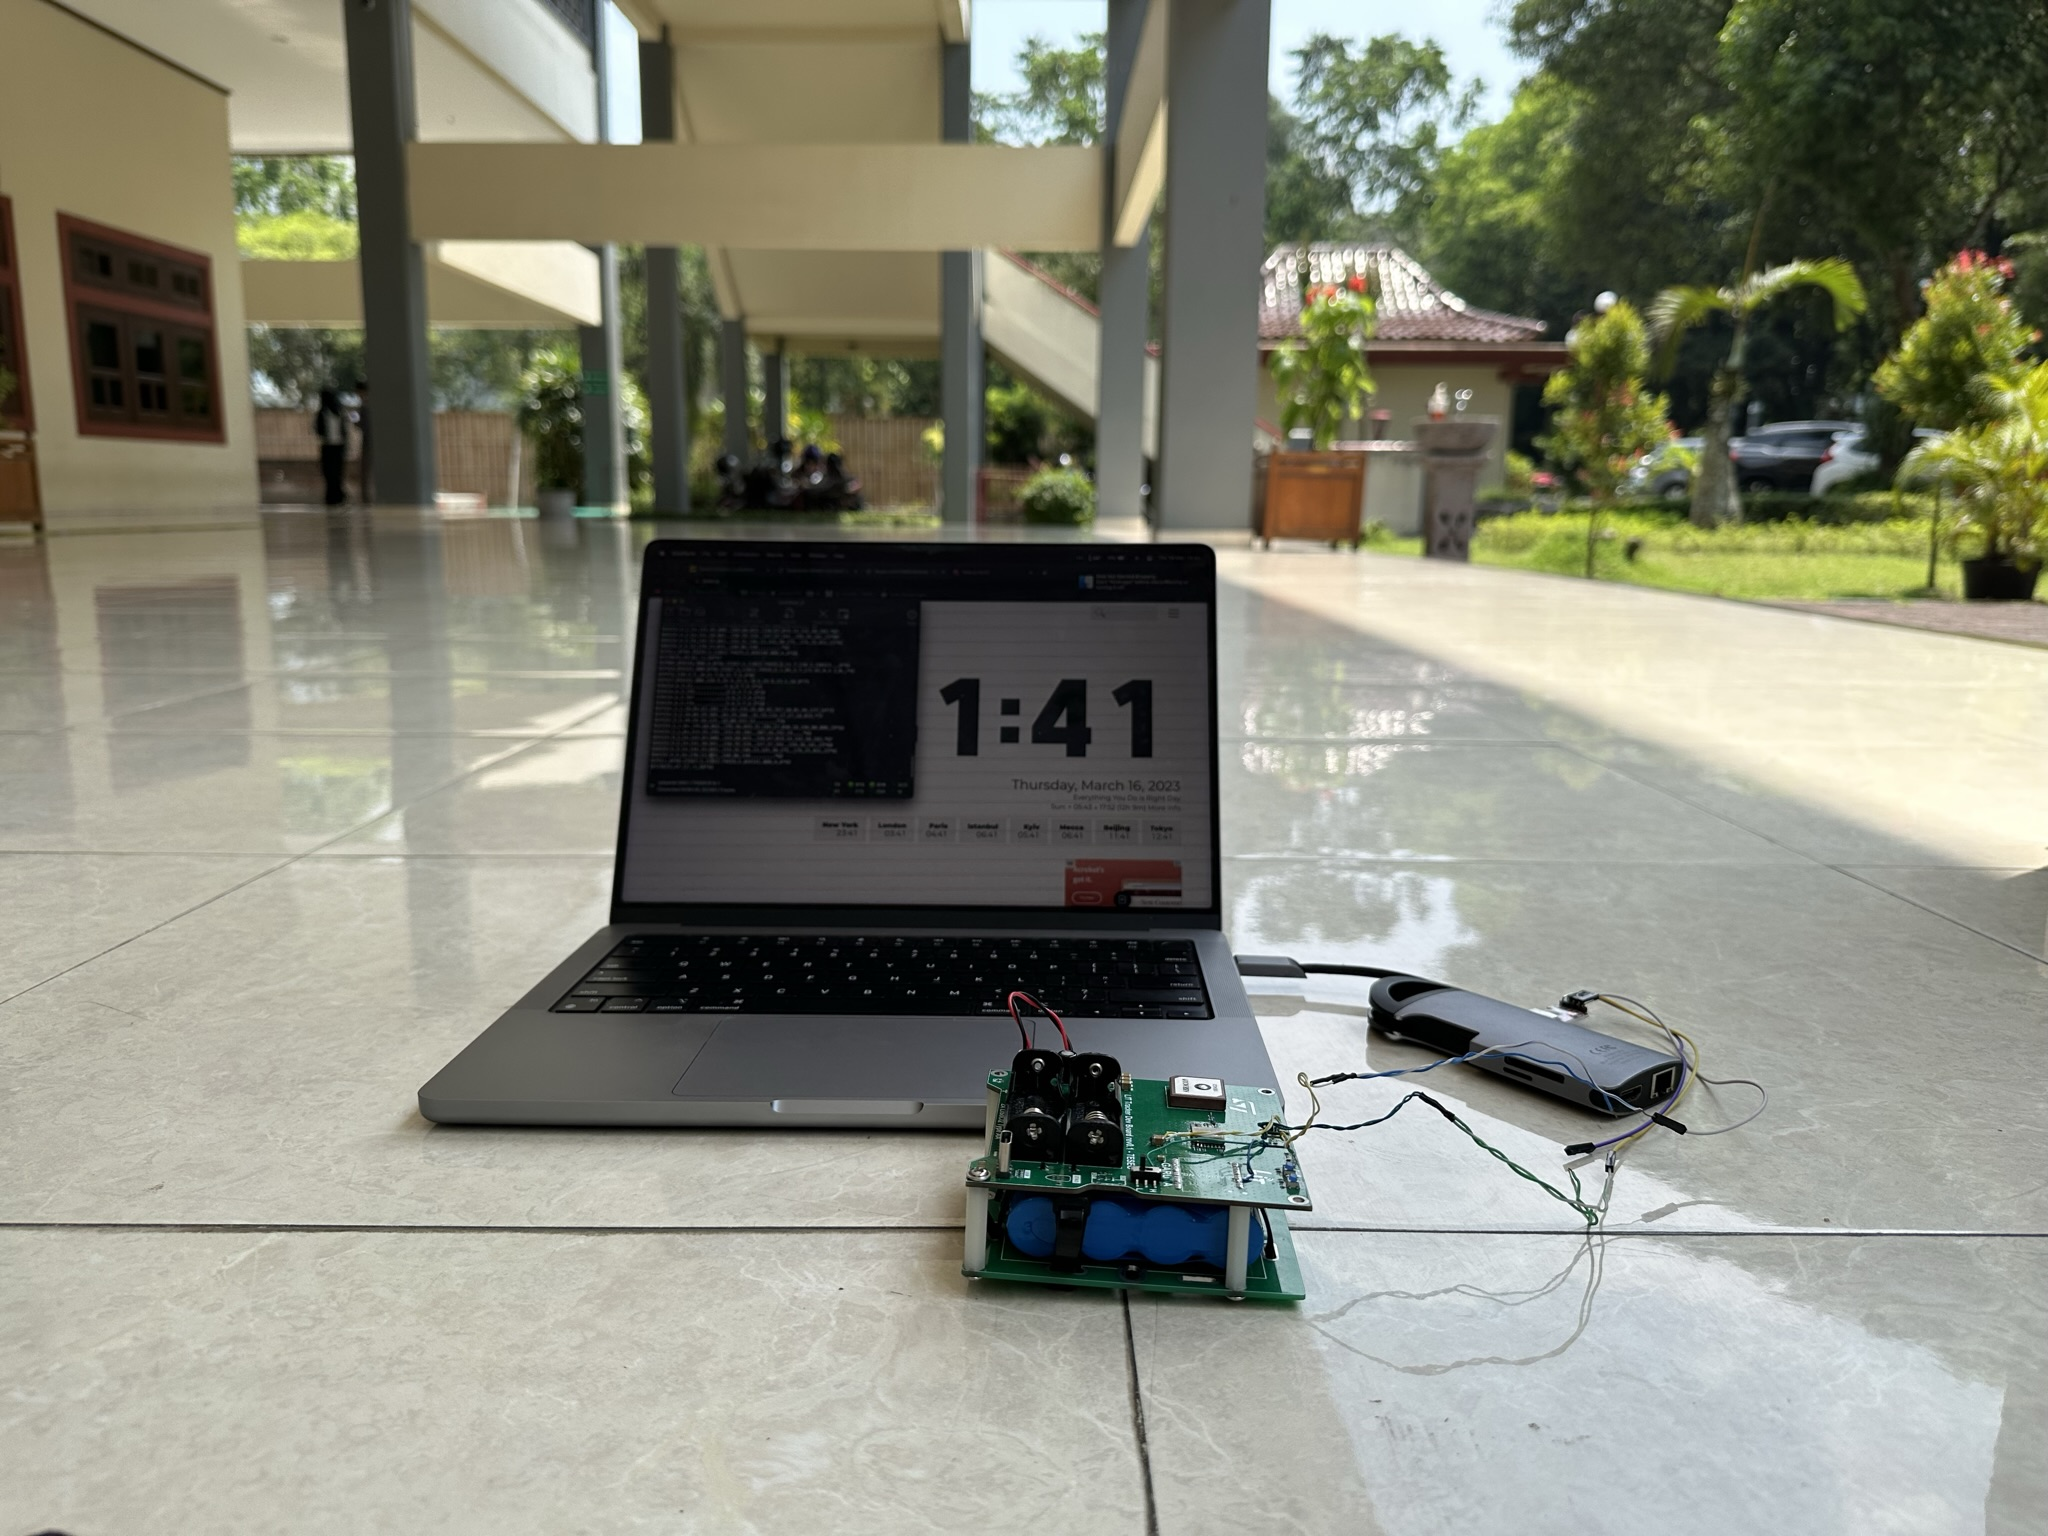
\includegraphics[width=10cm]{contents/chapter-4/3-skenario-semioutdoor/keadaan.jpeg}
	\caption{Pengujian Skenario Ruangan Semi Terbuka}
	\label{Fig: semioutdoor-keadaan}
\end{figure}

Pada pengujian ini, urutan konstelasi dengan jumlah satelit paling banyak hingga paling sedikit adalah GPS, BeiDou, QZSS, dan BeiDou. Rata-rata jumlah satelit yang digunakan adalah 14,32 dengan jumlah terbanyak 18 buah seperti ditunjukan pada Tabel \ref{Tab: semioutdoor-table}. Visibilitas satelit pada skenario ruangan semi terbuka lebih baik jika dibandingkan dengan dua skenario sebelumnya.

\begin{figure}[H]
	\centering
	\captionsetup{justification=centering}
	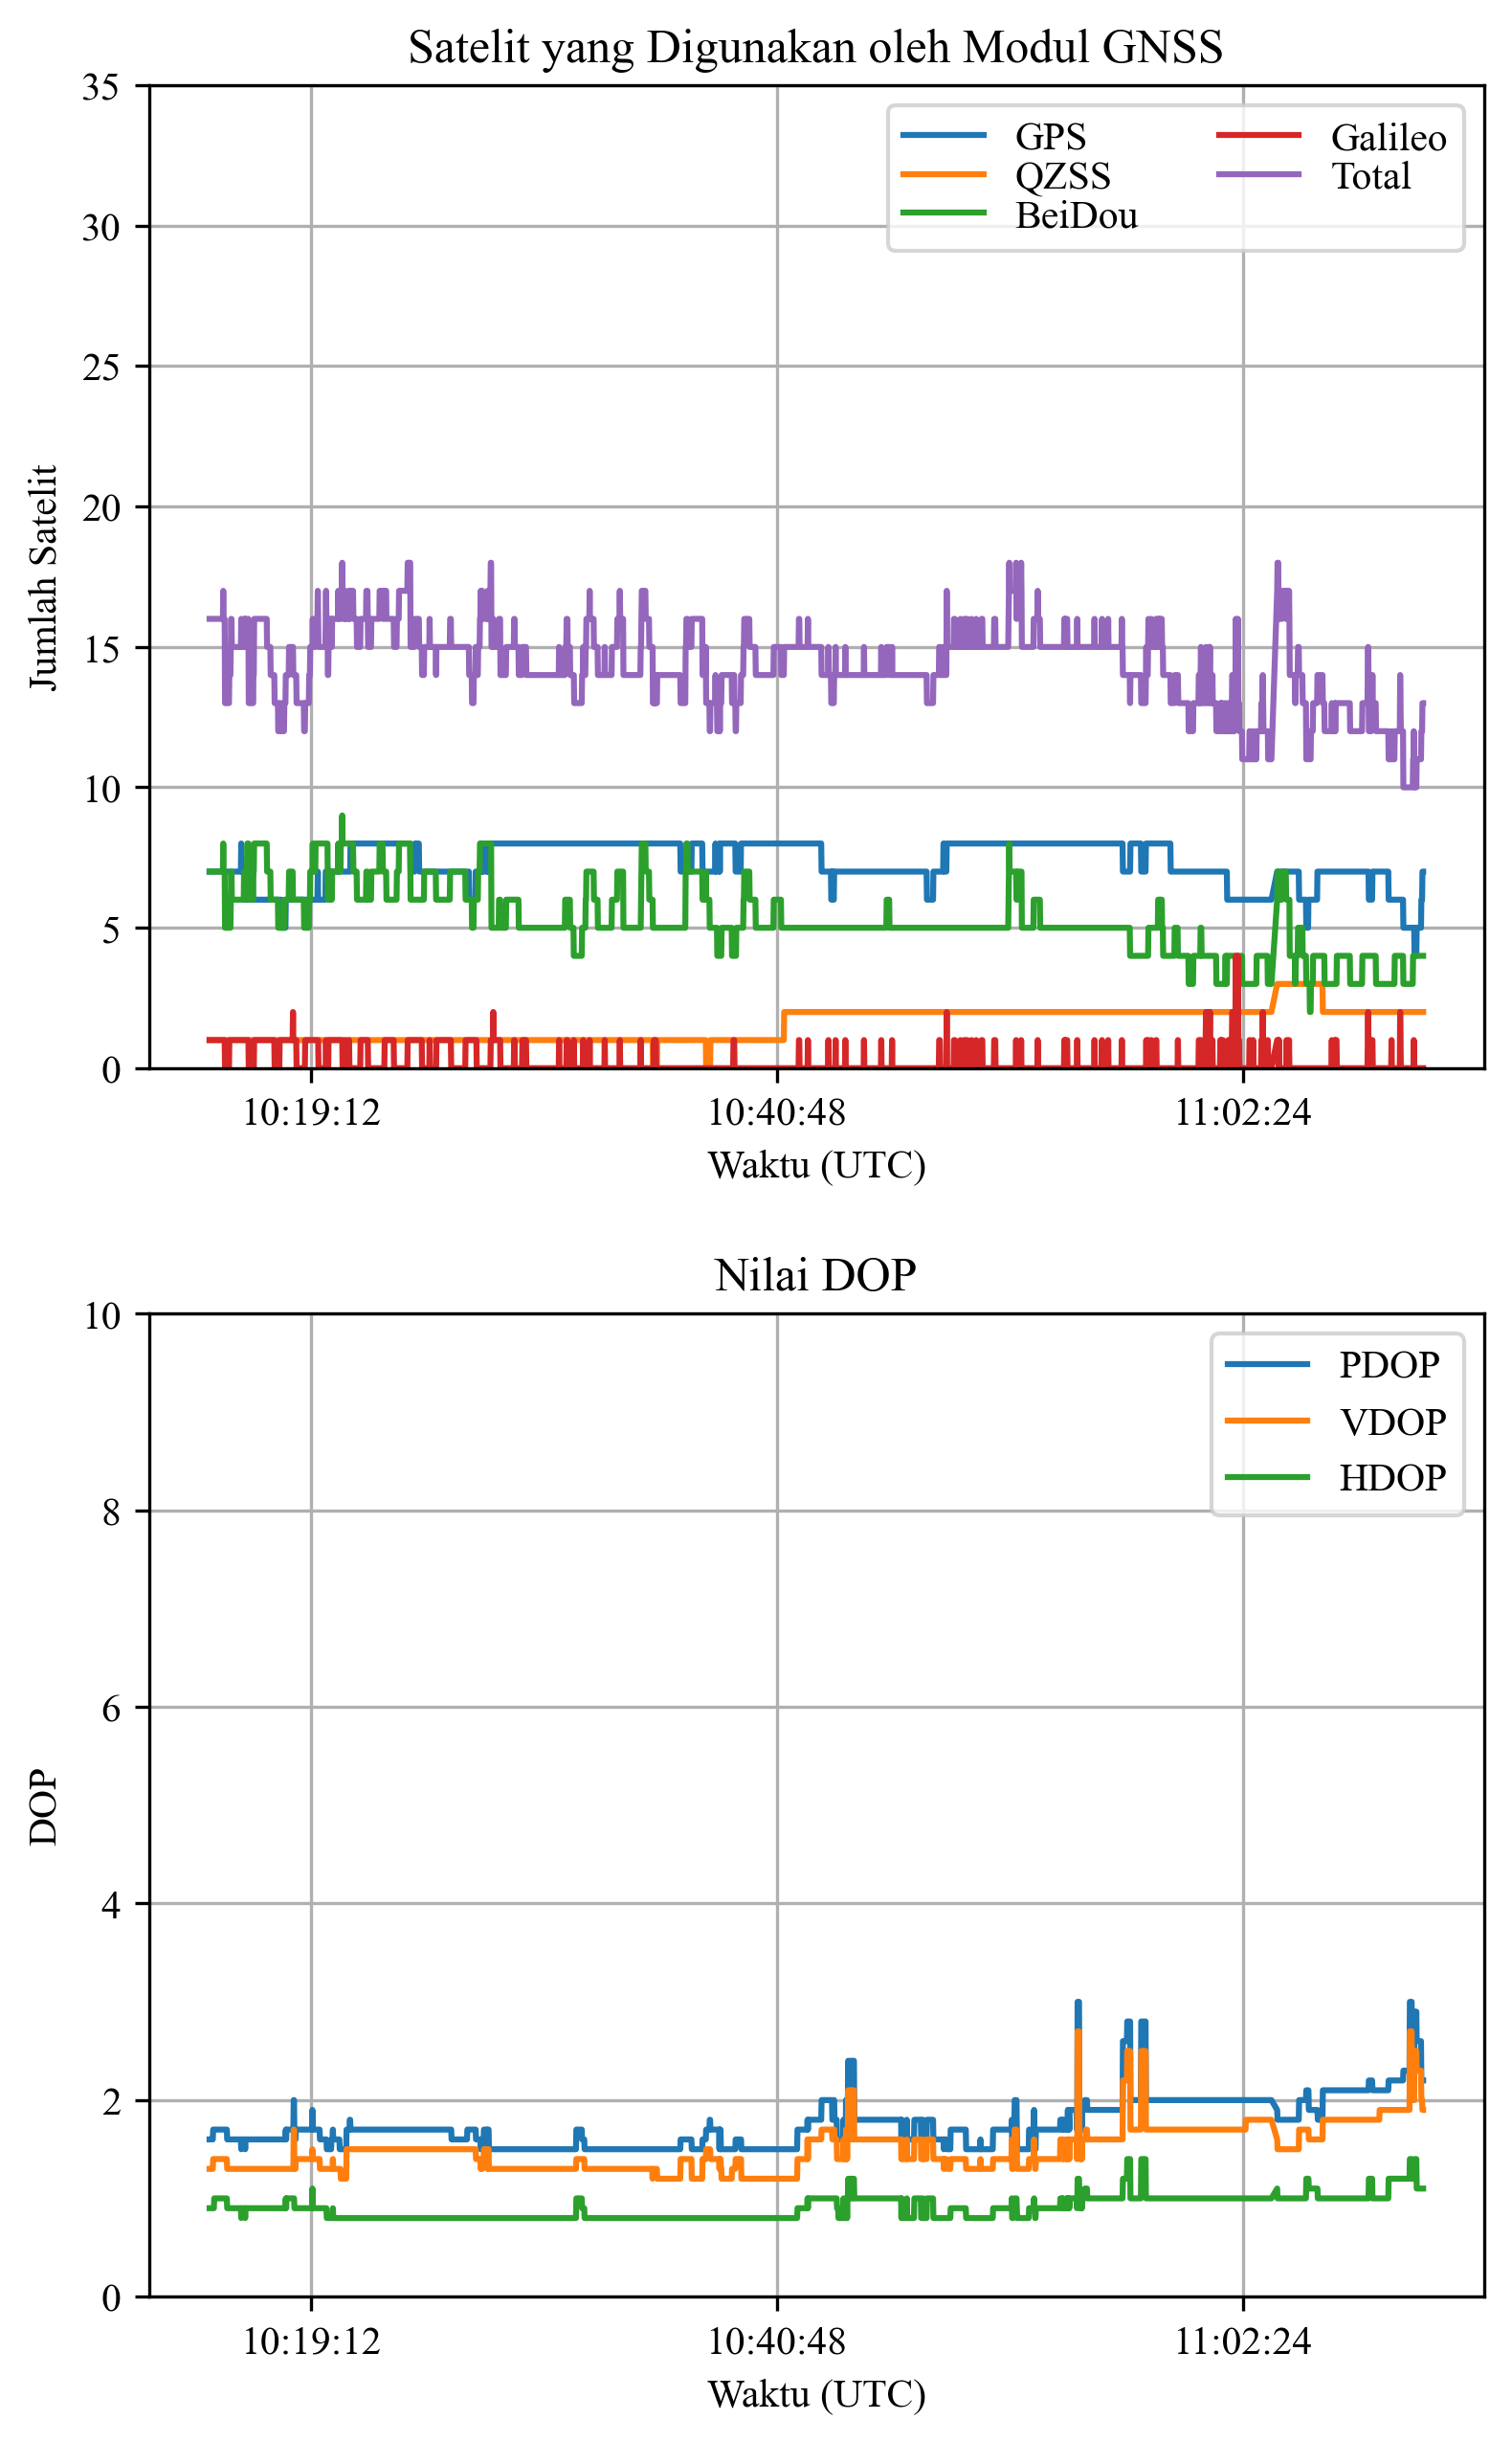
\includegraphics[width=11.5cm]{contents/chapter-4/3-skenario-semioutdoor/sats_dop.png}
	\caption{DOP dan Visibilitas Satelit Pengujian Skenario Ruangan Semi Terbuka}
	\label{Fig: semioutdoor-sats_dop}
\end{figure}

Jika ditinjau dari nilai DOP, ketiga nilai DOP juga mengalami penurunan secara signifikan. Penurunan nilai HDOP menunjukan terdapat peningkatan akurasi pada hasil pembacaan di bidang horizontal, sedangkan penurunan nilai VDOP menunjukan peningkatan akurasi pada pembacaan ketinggian. Gambar \ref{Fig: semioutdoor-sky_plot} menunjukan persebaran satelit di langit sudah mencakup seluruh kuadran lingkaran. Hal tersebut juga didukung oleh nilai PDOP yang lebih rendah.

\begin{figure}[H]
	\centering
	\captionsetup{justification=centering}
	\includegraphics[width=12cm]{contents/chapter-4/3-skenario-semioutdoor/sky_plot.png}
	\caption{\textit{Sky Plot} Skenario Ruangan Semi Terbuka}
	\label{Fig: semioutdoor-sky_plot}
\end{figure}

Pada skenario ini, rata-rata nilai CEP yang didapat adalah 13,83 m dengan nilai CEP terkecil adalah 7,28 m dan 28,32 m untuk nilai CEP terbesarnya. Berdasarkan hasil tersebut maka pada skenario ini terjadi penurunan CEP sebesar 1,68 m. Meskipun mengalami penurunan rata-rata pada nilai CEP-nya, tetapi perubahan nilai DOP-nya tidak sefluktuatif dua pengujian sebelumnya seperti ditunjukan oleh Gambar \ref{Fig: semioutdoor-sats_dop}.

Berdasarkan hasil yang didapat, pada pengujian skenario ini dapat dilihat bahwa penempatan modul Teseo-LIV3FL pada lingkungan dengan penghalang yang lebih sedikit dapat meningkatkan tingkat akurasinya. Rata-rata nilai PDOP dan VDOP sudah berada dalam rentang sangat baik dan HDOP berada dalam rentang ideal yang artinya sudah dapat digunakan dalam aplikasi yang sensitif terhadap ketelitian. Penurunan rata-rata nilai CEP tidak terlalu signifikan jika dibandingkan dengan pengujian pada skenario \textit{basement}.

\subsection{Skenario Ruangan Terbuka}
\begin{table}[H]
	\caption{Hasil Pengujian Ruangan Terbuka}
	\vspace{0.5em}
	\centering
	\begin{tabular}{ccccc}
		\hline
		& \textbf{Minima} & \textbf{Maxima} & \textbf{Rata-rata} & \textbf{Standar Deviasi}\\
		\hline 
		HDOP & 0,60 & 0,80 & 0,65 & 0,06 \\
		PDOP & 0,90 & 1,60 & 1,12 & 0,15 \\
		VDOP & 1,10	& 1,80 & 1,30 & 0,15 \\
		CEP (m) & 5,22 & 6,80 & 6,12 & 0,41 \\
		Jumlah Satelit & 17	& 25 & 21,14 & 1,37 \\
		\hline
	\end{tabular}
	\label{Tab: outdoor-table}
\end{table}

Pengujian skenario ruangan terbuka bertujuan untuk meninjau performa modul Teseo-LIV3FL di ruangan terbuka. Titik pengujian berada di Lapangan Pancasila Universitas Gadjah Mada dengan kondisi langit cerah. Pemilihan lokasi Lapangan Pancasila bertujuan untuk meminimalisasi penghalang seperti gedung dan pepohonan. Gambar \ref{Fig: outdoor-keadaan} menunjukan pengujian skenasio ruangan terbuka.

\begin{figure}[H]
	\centering
	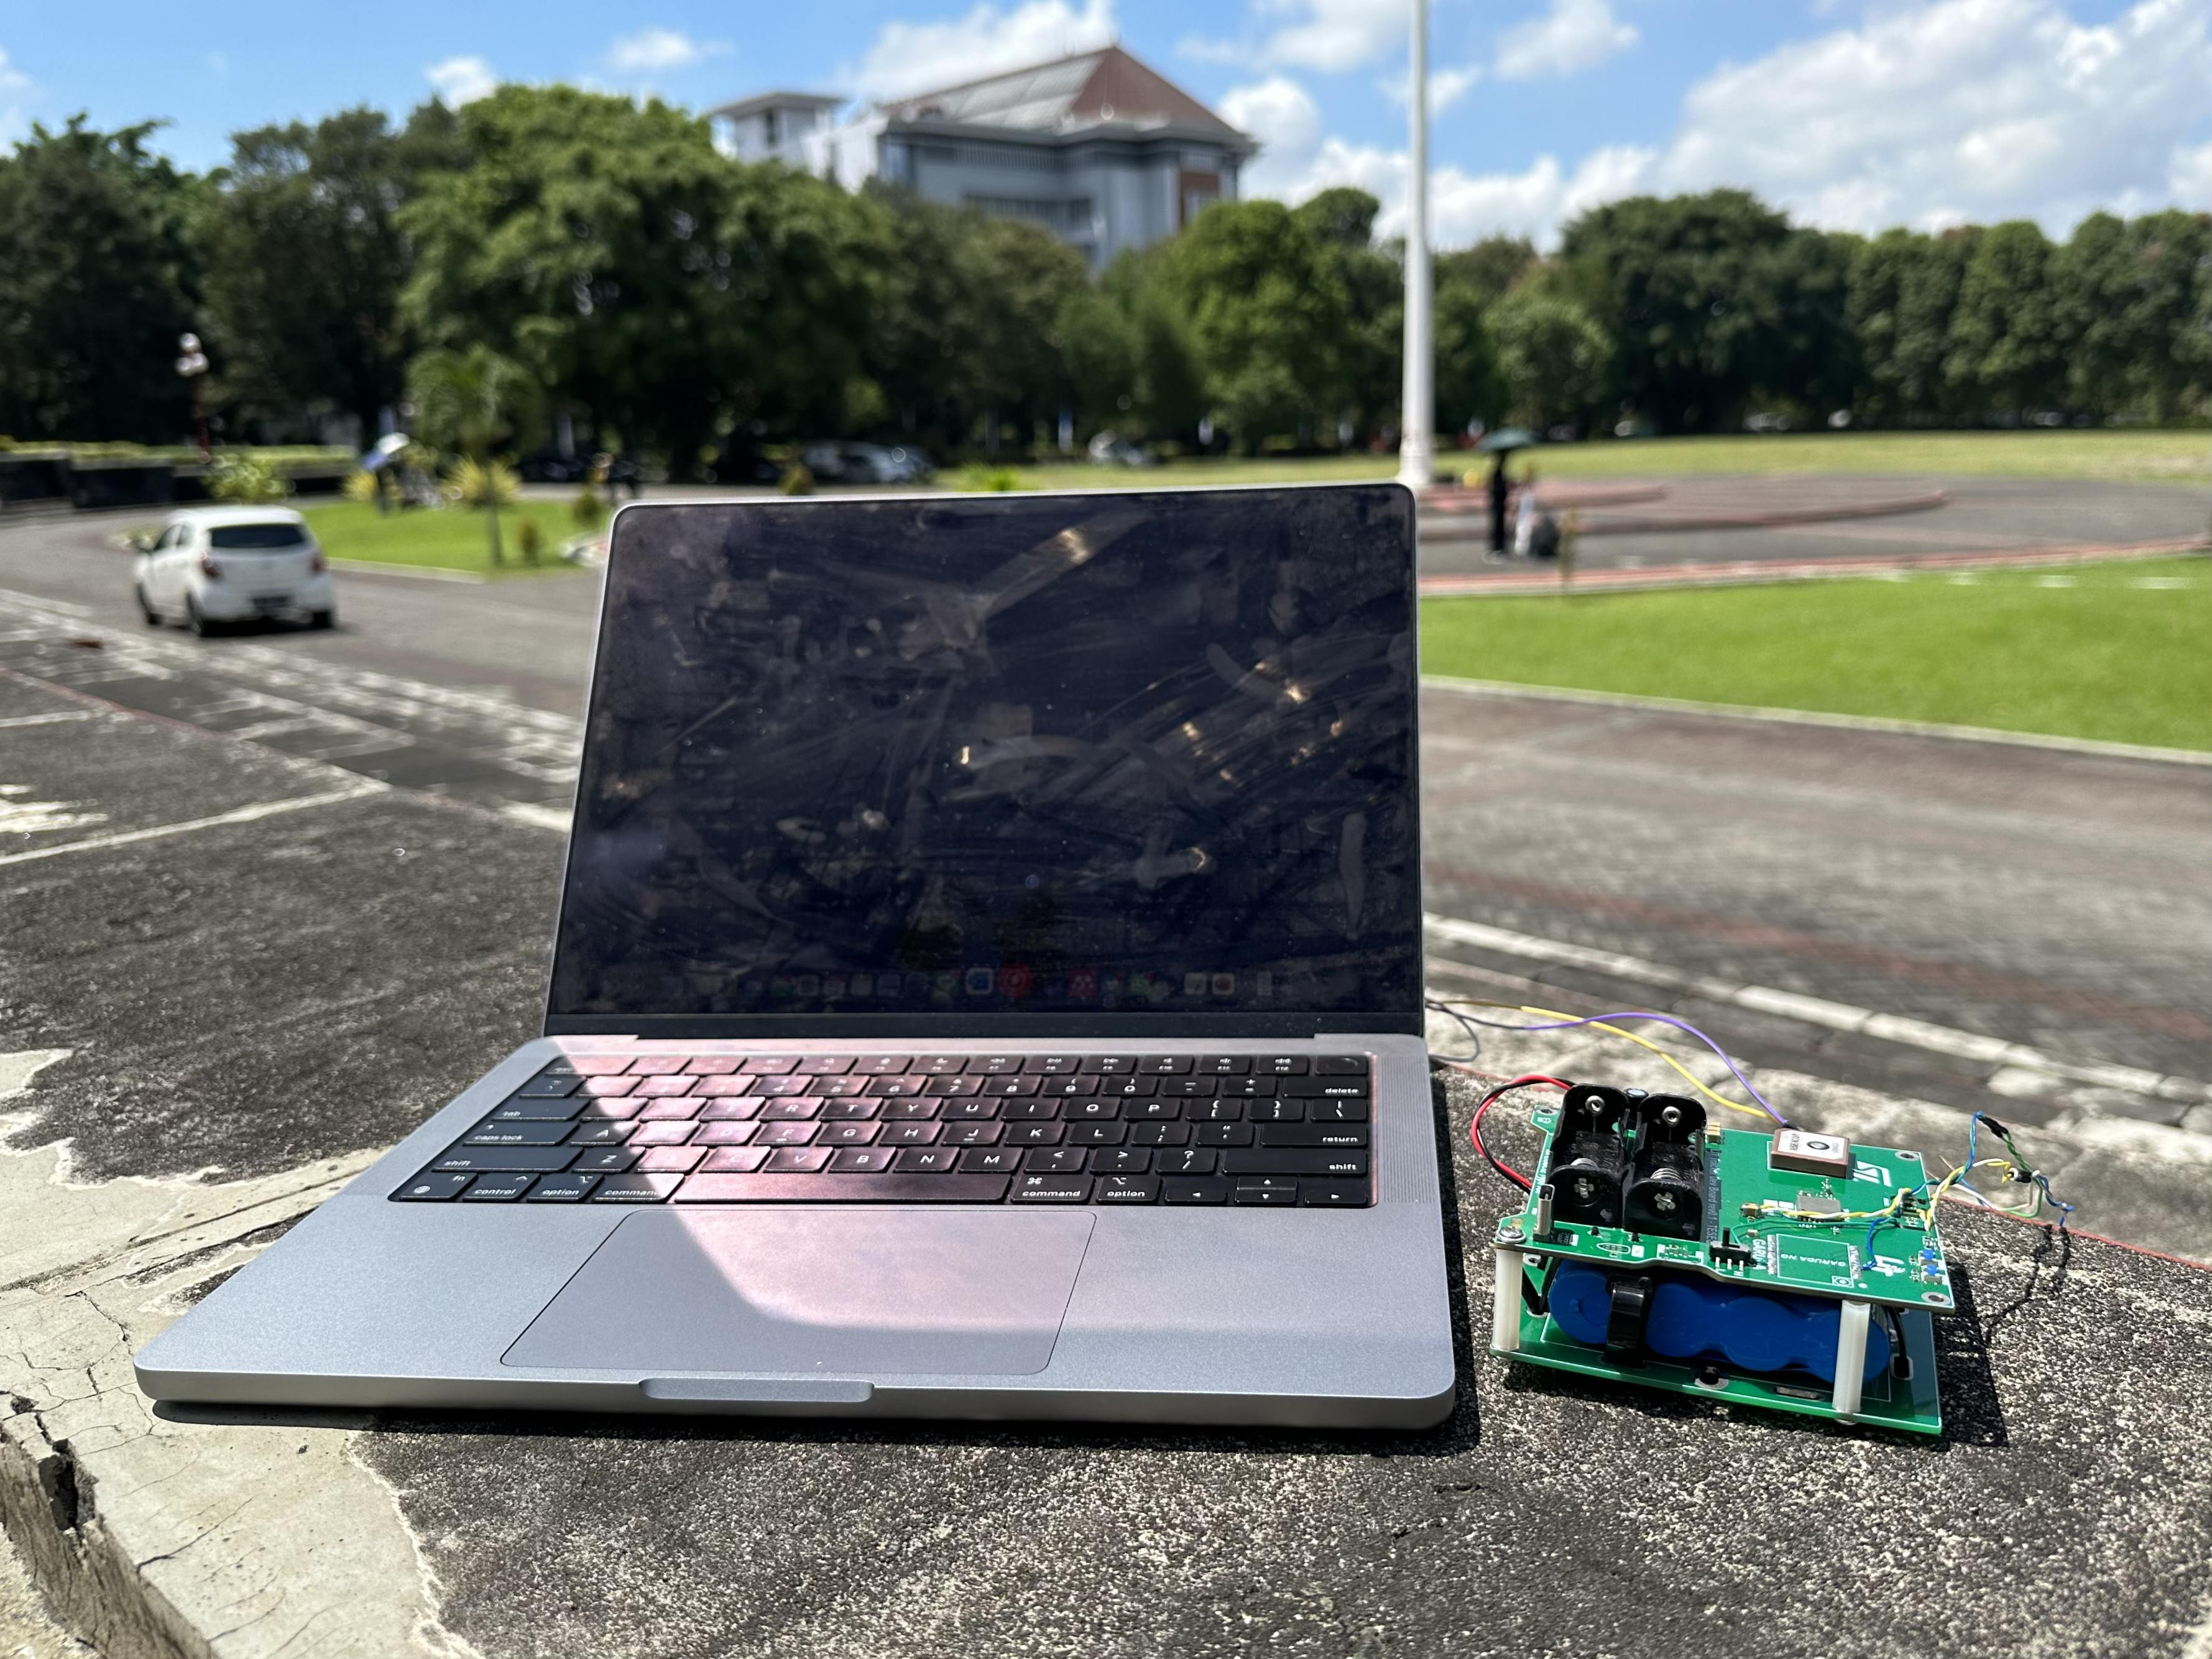
\includegraphics[width=10cm]{contents/chapter-4/4-skenario-outdoor/keadaan.jpg}
	\caption{Pengujian Skenario Ruang Terbuka}
	\label{Fig: outdoor-keadaan}
\end{figure}

Tabel \ref{Tab: outdoor-table} menunjukan bahwa pada skenario ruang terbuka memberikan hasil akurasi yang lebih tinggi. Rata-rata nilai DOP yang didapat berada pada rentang sangat baik s.d. ideal. Rata-rata nilai PDOP yang didapat adalah sebesar 1,12 dengan PDOP terkecil adalah 0,90 dan terbesarnya 1,60. Nilai PDOP yang kecil didukung oleh persebaran satelit di langit yang lebih banyak mencakup bagian lingkaran pada Gambar \ref{Fig: outdoor-skyplot}.

\begin{figure}[H]
	\centering
	\includegraphics[width=12cm]{contents/chapter-4/4-skenario-outdoor/sky_plot.png}
	\caption{\textit{Sky Plot} Pengujian Ruang Terbuka}
	\label{Fig: outdoor-skyplot}
\end{figure}

Pada skenario ruang terbuka, didapat nilai CEP paling rendah dari seluruh pengujian \textit{rapid static survey} dengan rata-rata nilai CEP 6,12 m. Selain itu, visibilitas satelit maksimum juga didapat pada pengujian ini dengan jumlah satelit paling banyak sebanyak dua puluh lima buah satelit. Gambar \ref{Fig: outdoor-dop_sats} menunjukan konstelasi dengan jumlah satelit paling banyak adalah BeiDou yang kemudian disusul oleh GPS, QZSS, dan Galileo. 

\begin{figure}[H]
	\centering
	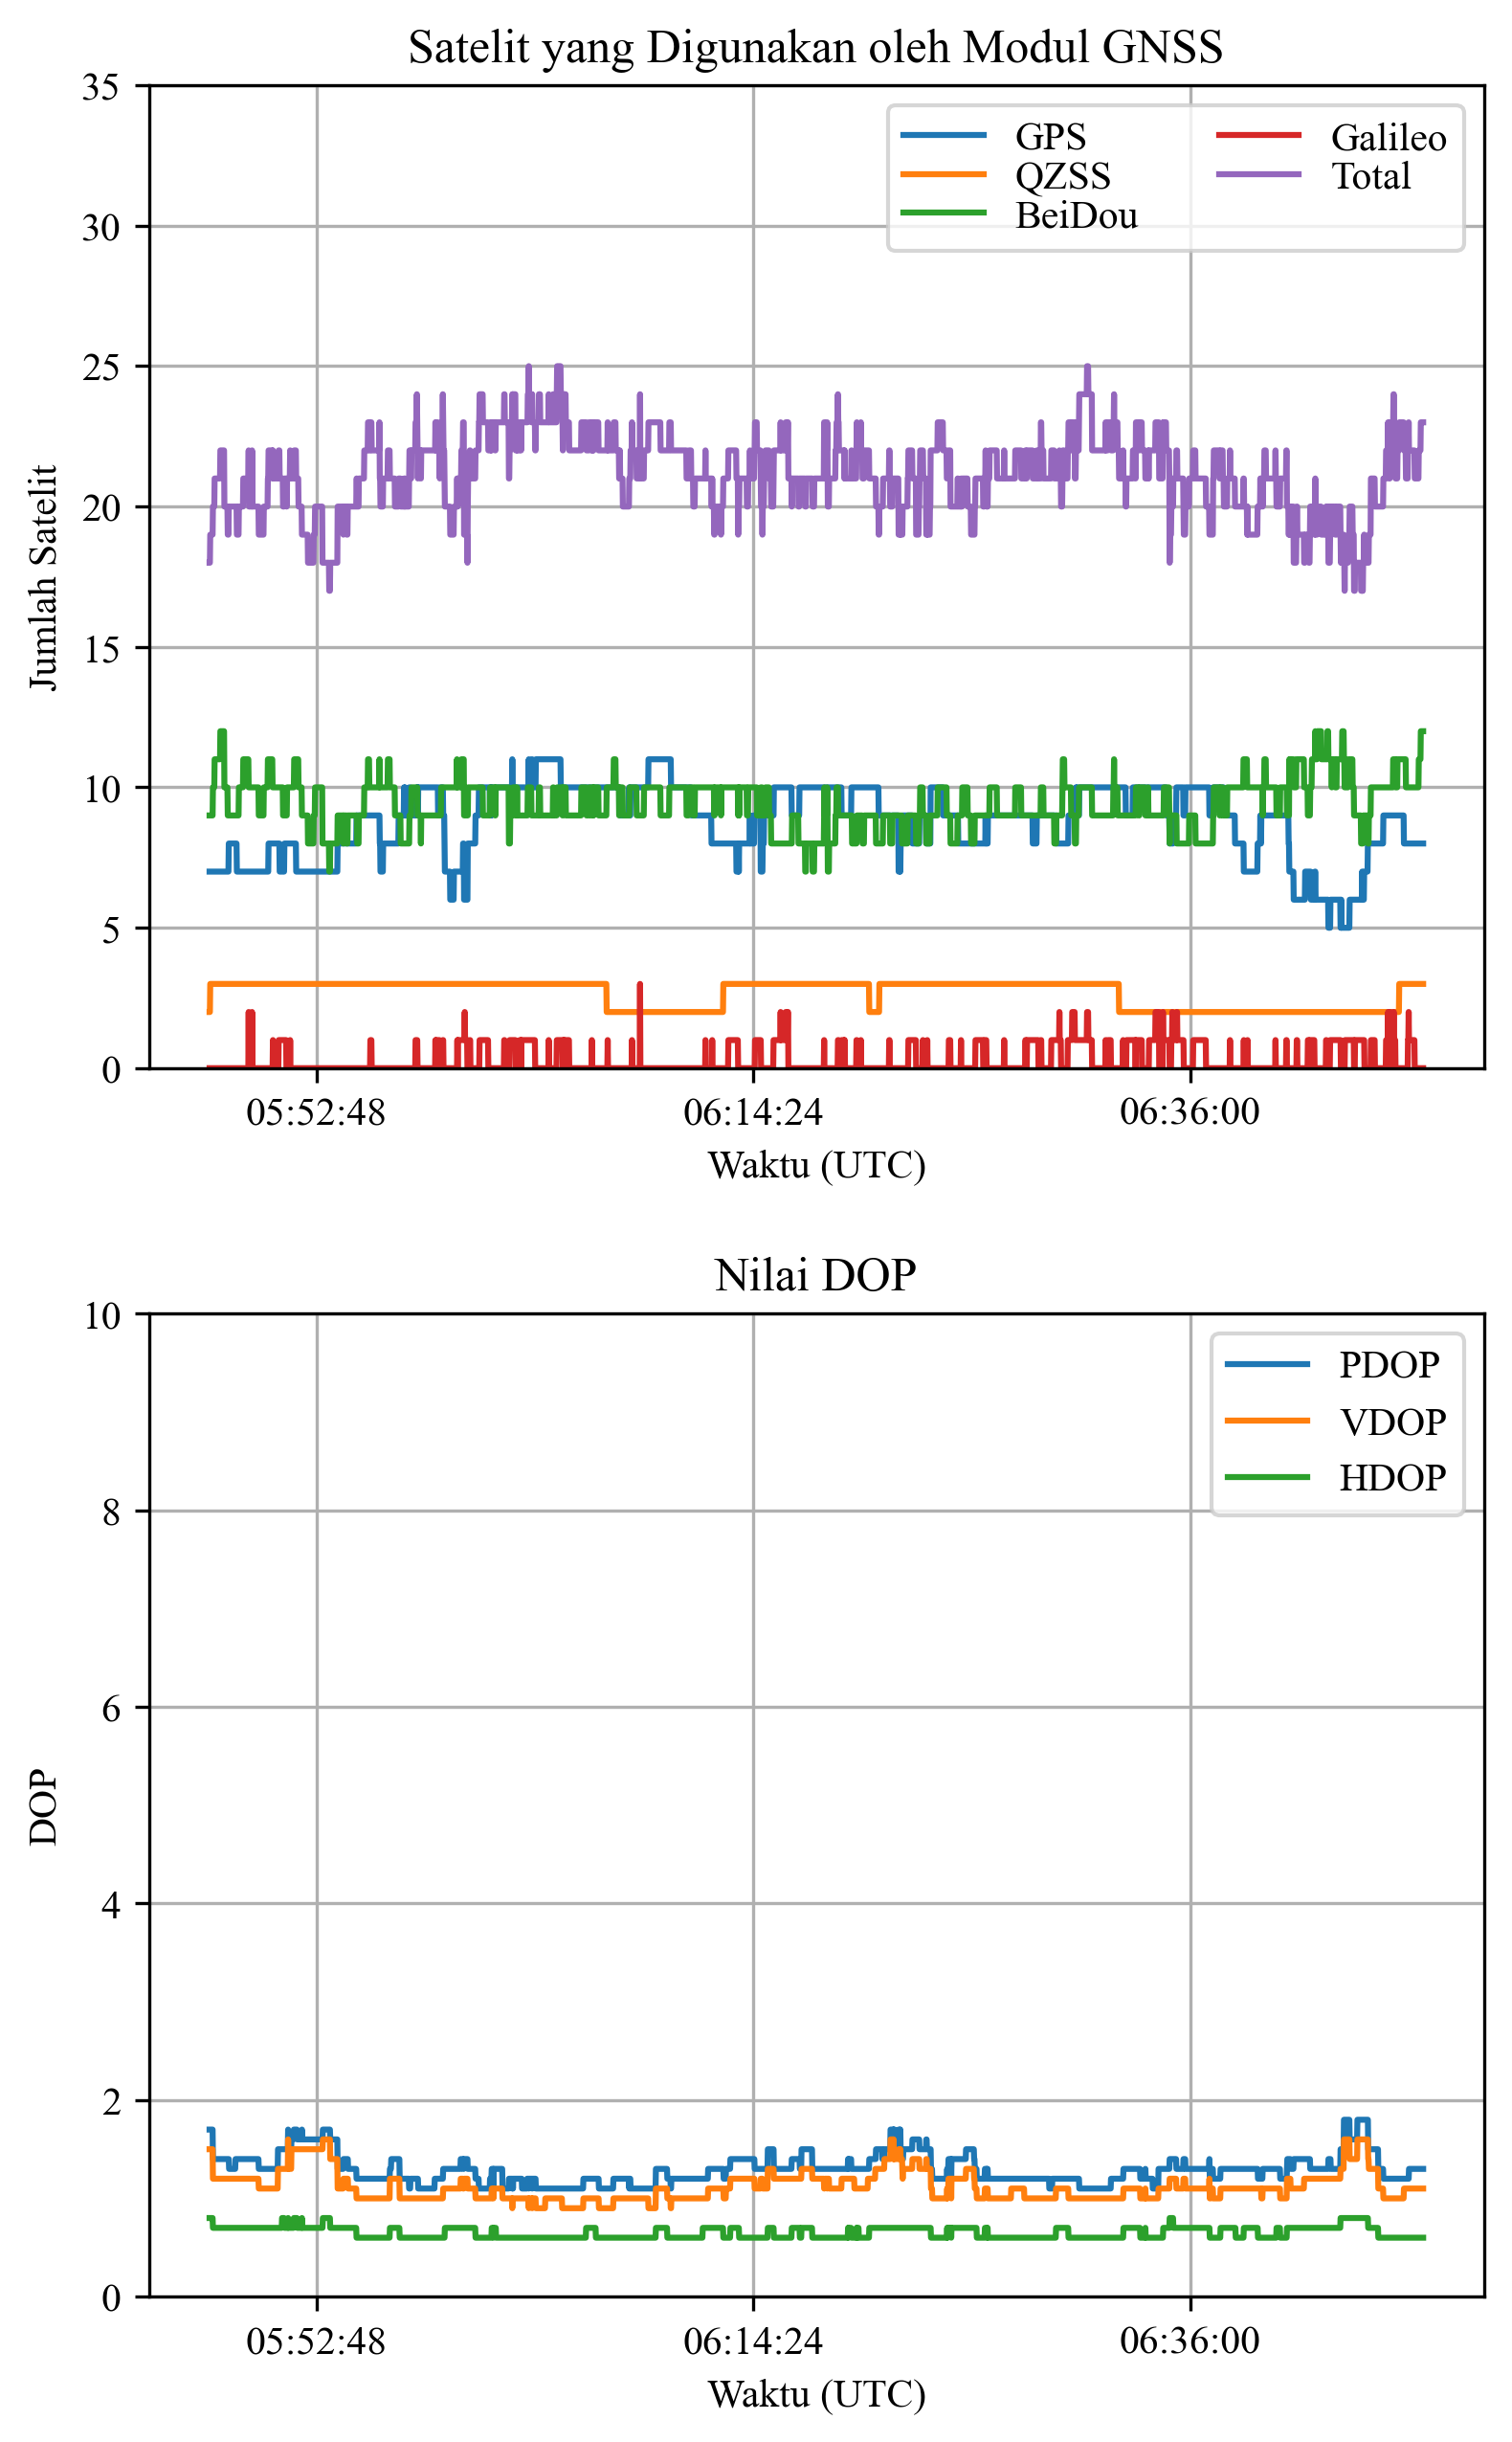
\includegraphics[width=12cm]{contents/chapter-4/4-skenario-outdoor/sats_dop.png}
	\caption{DOP dan Visibilitas Satelit Pengujian Pengujian Ruang Terbuka}
	\label{Fig: outdoor-dop_sats}
\end{figure}

Hasil pengujian menunjukan bahwa skenario ruang terbuka memberikan hasil pengukuran paling baik jika dibandingkan dengan tiga pengujian sebelumnya. Meskipun tidak ada perubahan signifikan pada akurasi modul Teseo-LIV3FL, tetapi penurunan nilai CEP hingga 7,71 m menunjukan peningkatkan tingkat presisi yang sangat signifikan. Berdasarkan empat skenario pengujian yang telah dilakukan, untuk mendapat hasil yang maksimal maka modul Teseo-LIV3FL diletakan di ruang terbuka dengan keadaan langit cerah.

\section{Pengujian di Bus Trans Gadjah Mada}
Pengujian di Bus Trans Gadjah Mada dilakukan untuk meninjau performa sistem dalam keadaan bergerak. Sistem diletakan di dalam kendaraan bus yang terbuat dari logam. Rute pengujian mengikuti rute 1B Trans Gadjah Mada yang dimulai dari Halte Grha Sabha Pramana hingga kembali lagi ke Halte Grha Sabha Pramana dengan durasi waktu satu jam. Peta dari Trans Gadjah Mada Rute 1B ditunjukan oleh Gambar \ref{Fig: peta-1b}.

\begin{figure}[H]
	\centering
	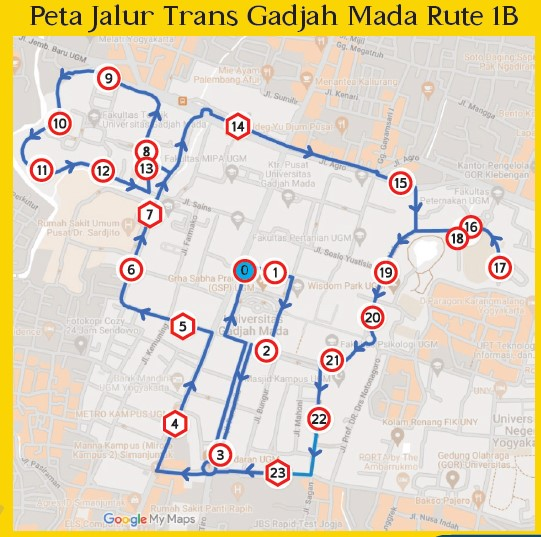
\includegraphics[width=10cm]{contents/chapter-4/pengujian-bergerak/Peta-Jalur-Rute-1B.jpg}
	\caption{Peta Jalur Trans Gadjah Mada Rute 1B}
	\label{Fig: peta-1b}
\end{figure}

Gambar \ref{Fig: moving-dop} menunjukan nilai DOP di setiap titik yang direpresentasikan oleh kode warna di sebelah kanan. Jika warna dari poin semakin mendekati warna merah maka nilai DOP-nya semakin buruk (mendekati 99). 

\begin{figure}[H]
	\centering
	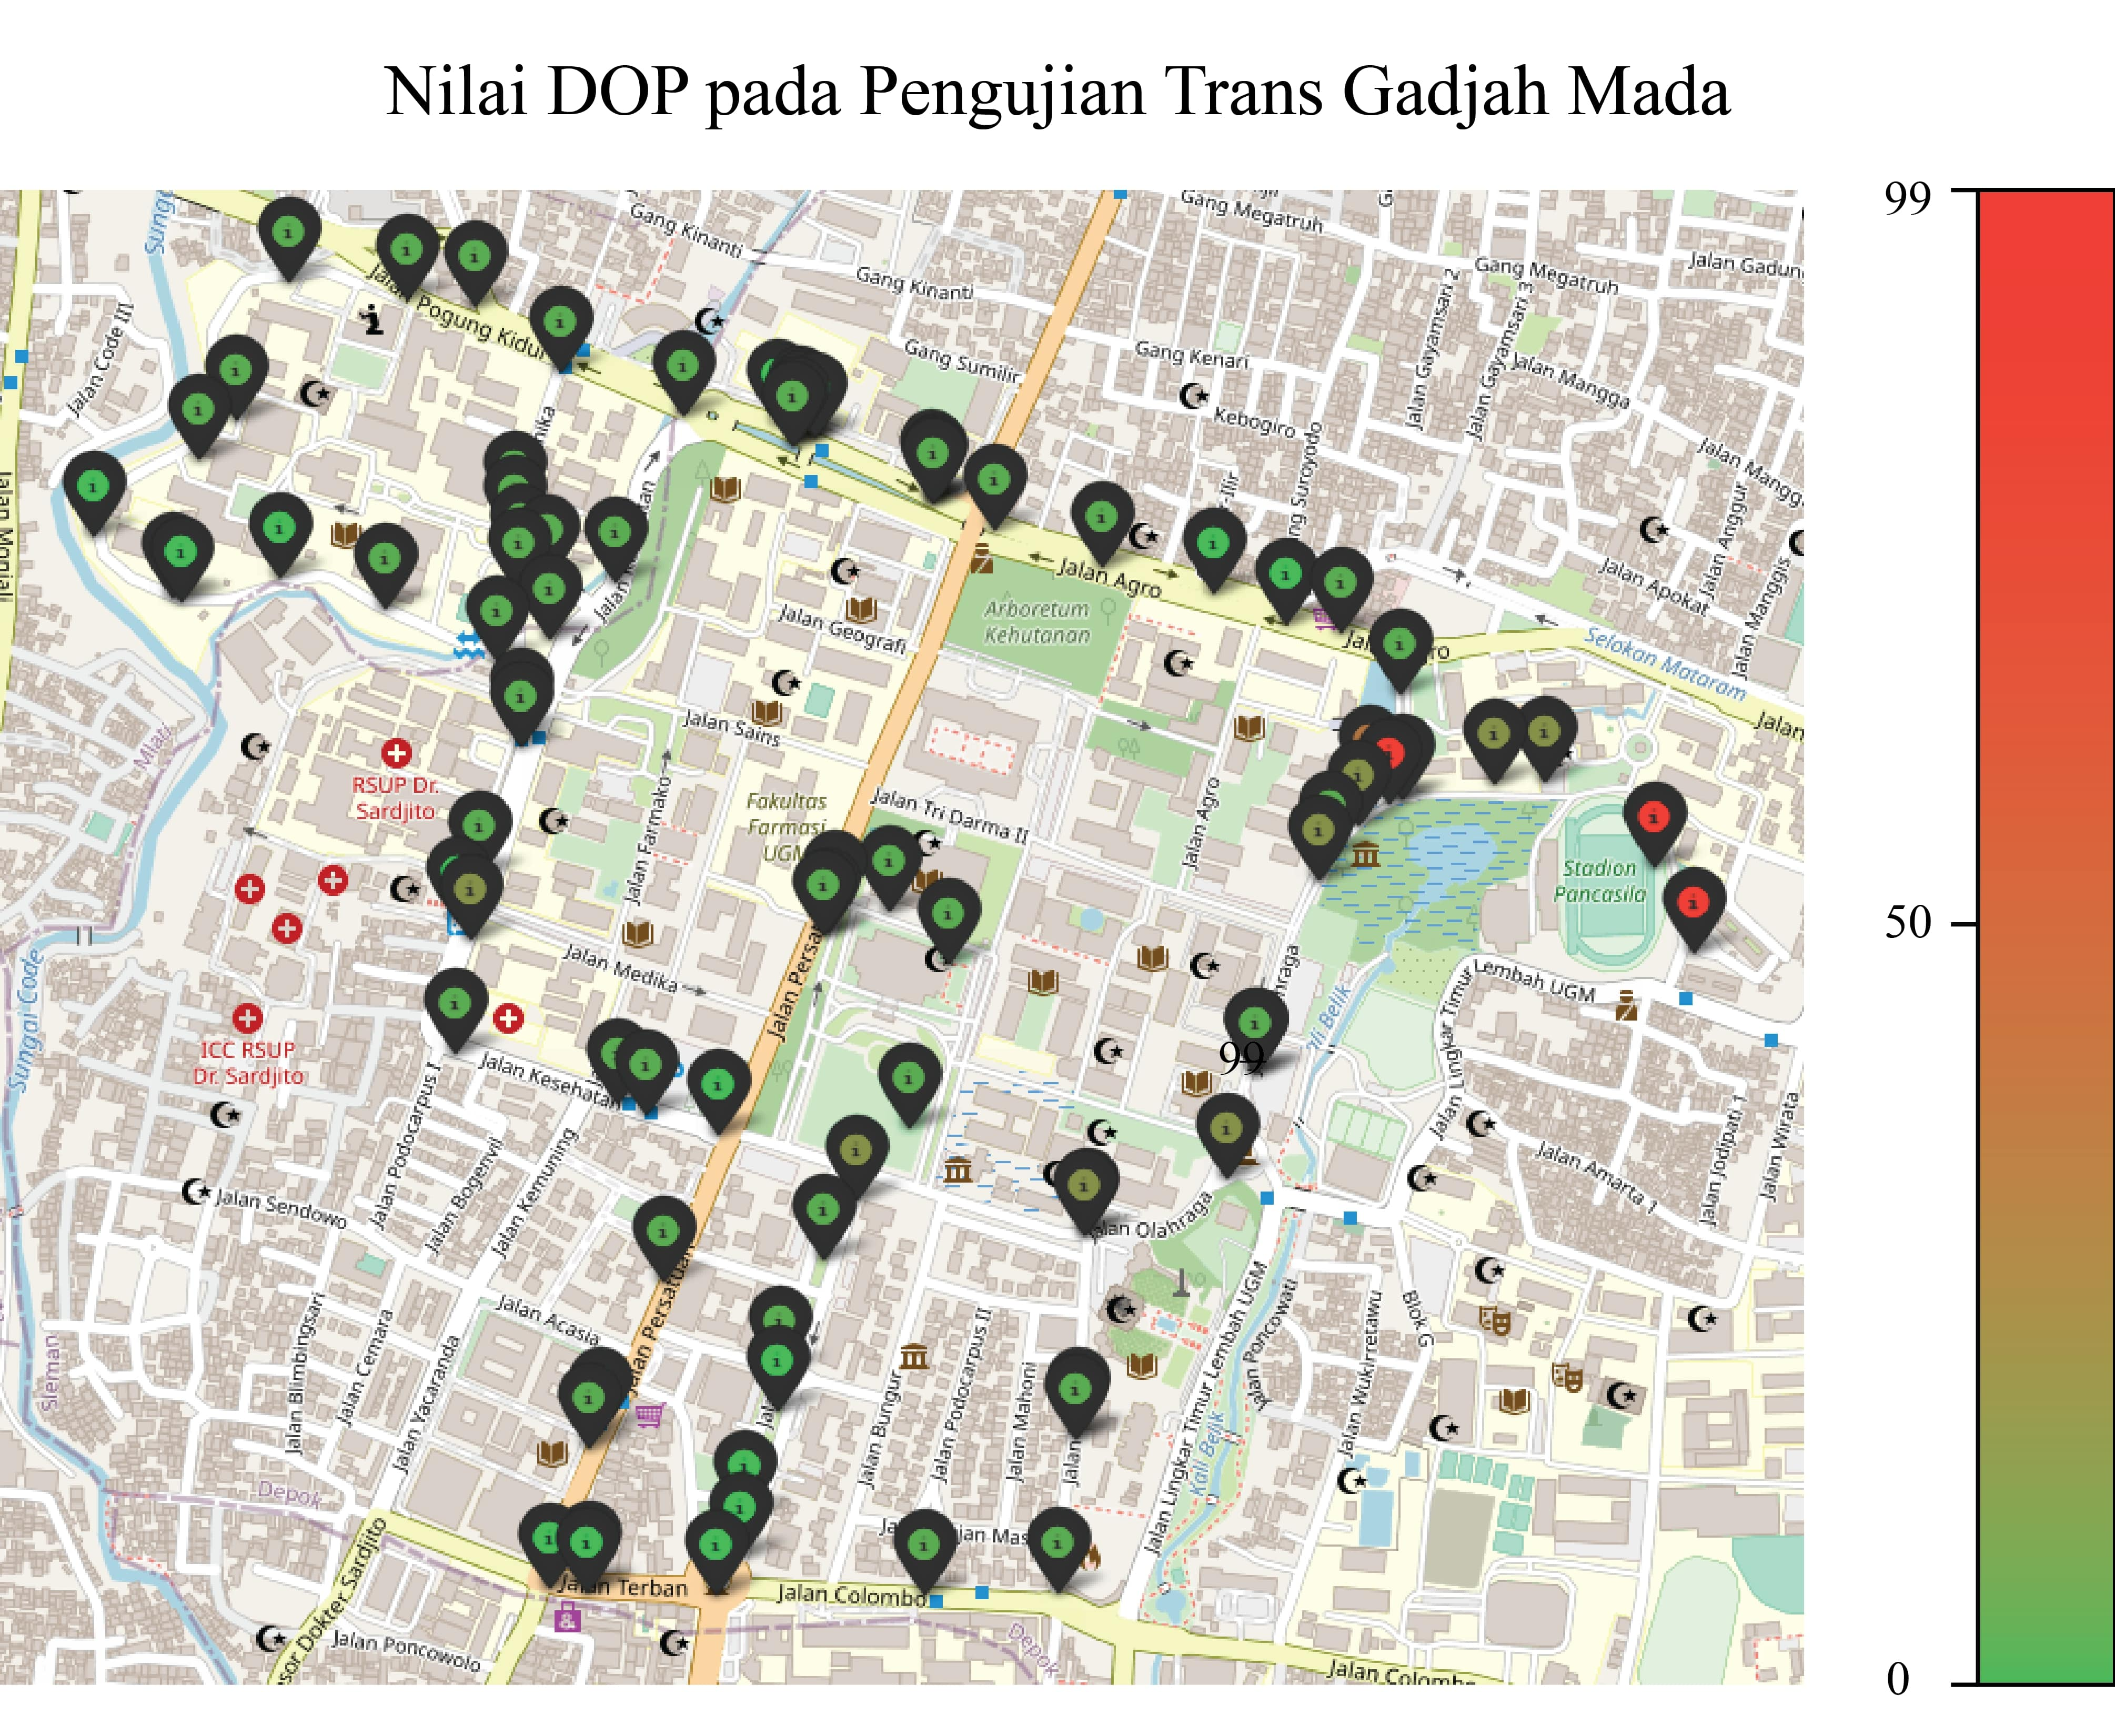
\includegraphics[width=12cm]{contents/chapter-4/pengujian-bergerak/moving-dop.jpg}
	\caption{Pengujian Skenario Dalam Ruangan}
	\label{Fig: moving-dop}
\end{figure}

Terlihat bahwa nilai DOP berada di rentang sangat buruk ketika berada di sekitar Bulaksumur Residence dan Stadion Pancasila. Hal tersebut dikarenakan lingkungan di sekitar pengujian banyak ditutupi oleh pepohonan dan terdapat beberapa gedung seperti ditunjukan oleh Gambar \ref{Fig: lp-streetview}. Halangan-halangan tersebut dapat mengurangi visibilitas dari satelit sehingga mengurangi akurasi dari modul GNSS yang mengakibatkan lonjakan nilai DOP.

\begin{figure}[H]
	\centering
	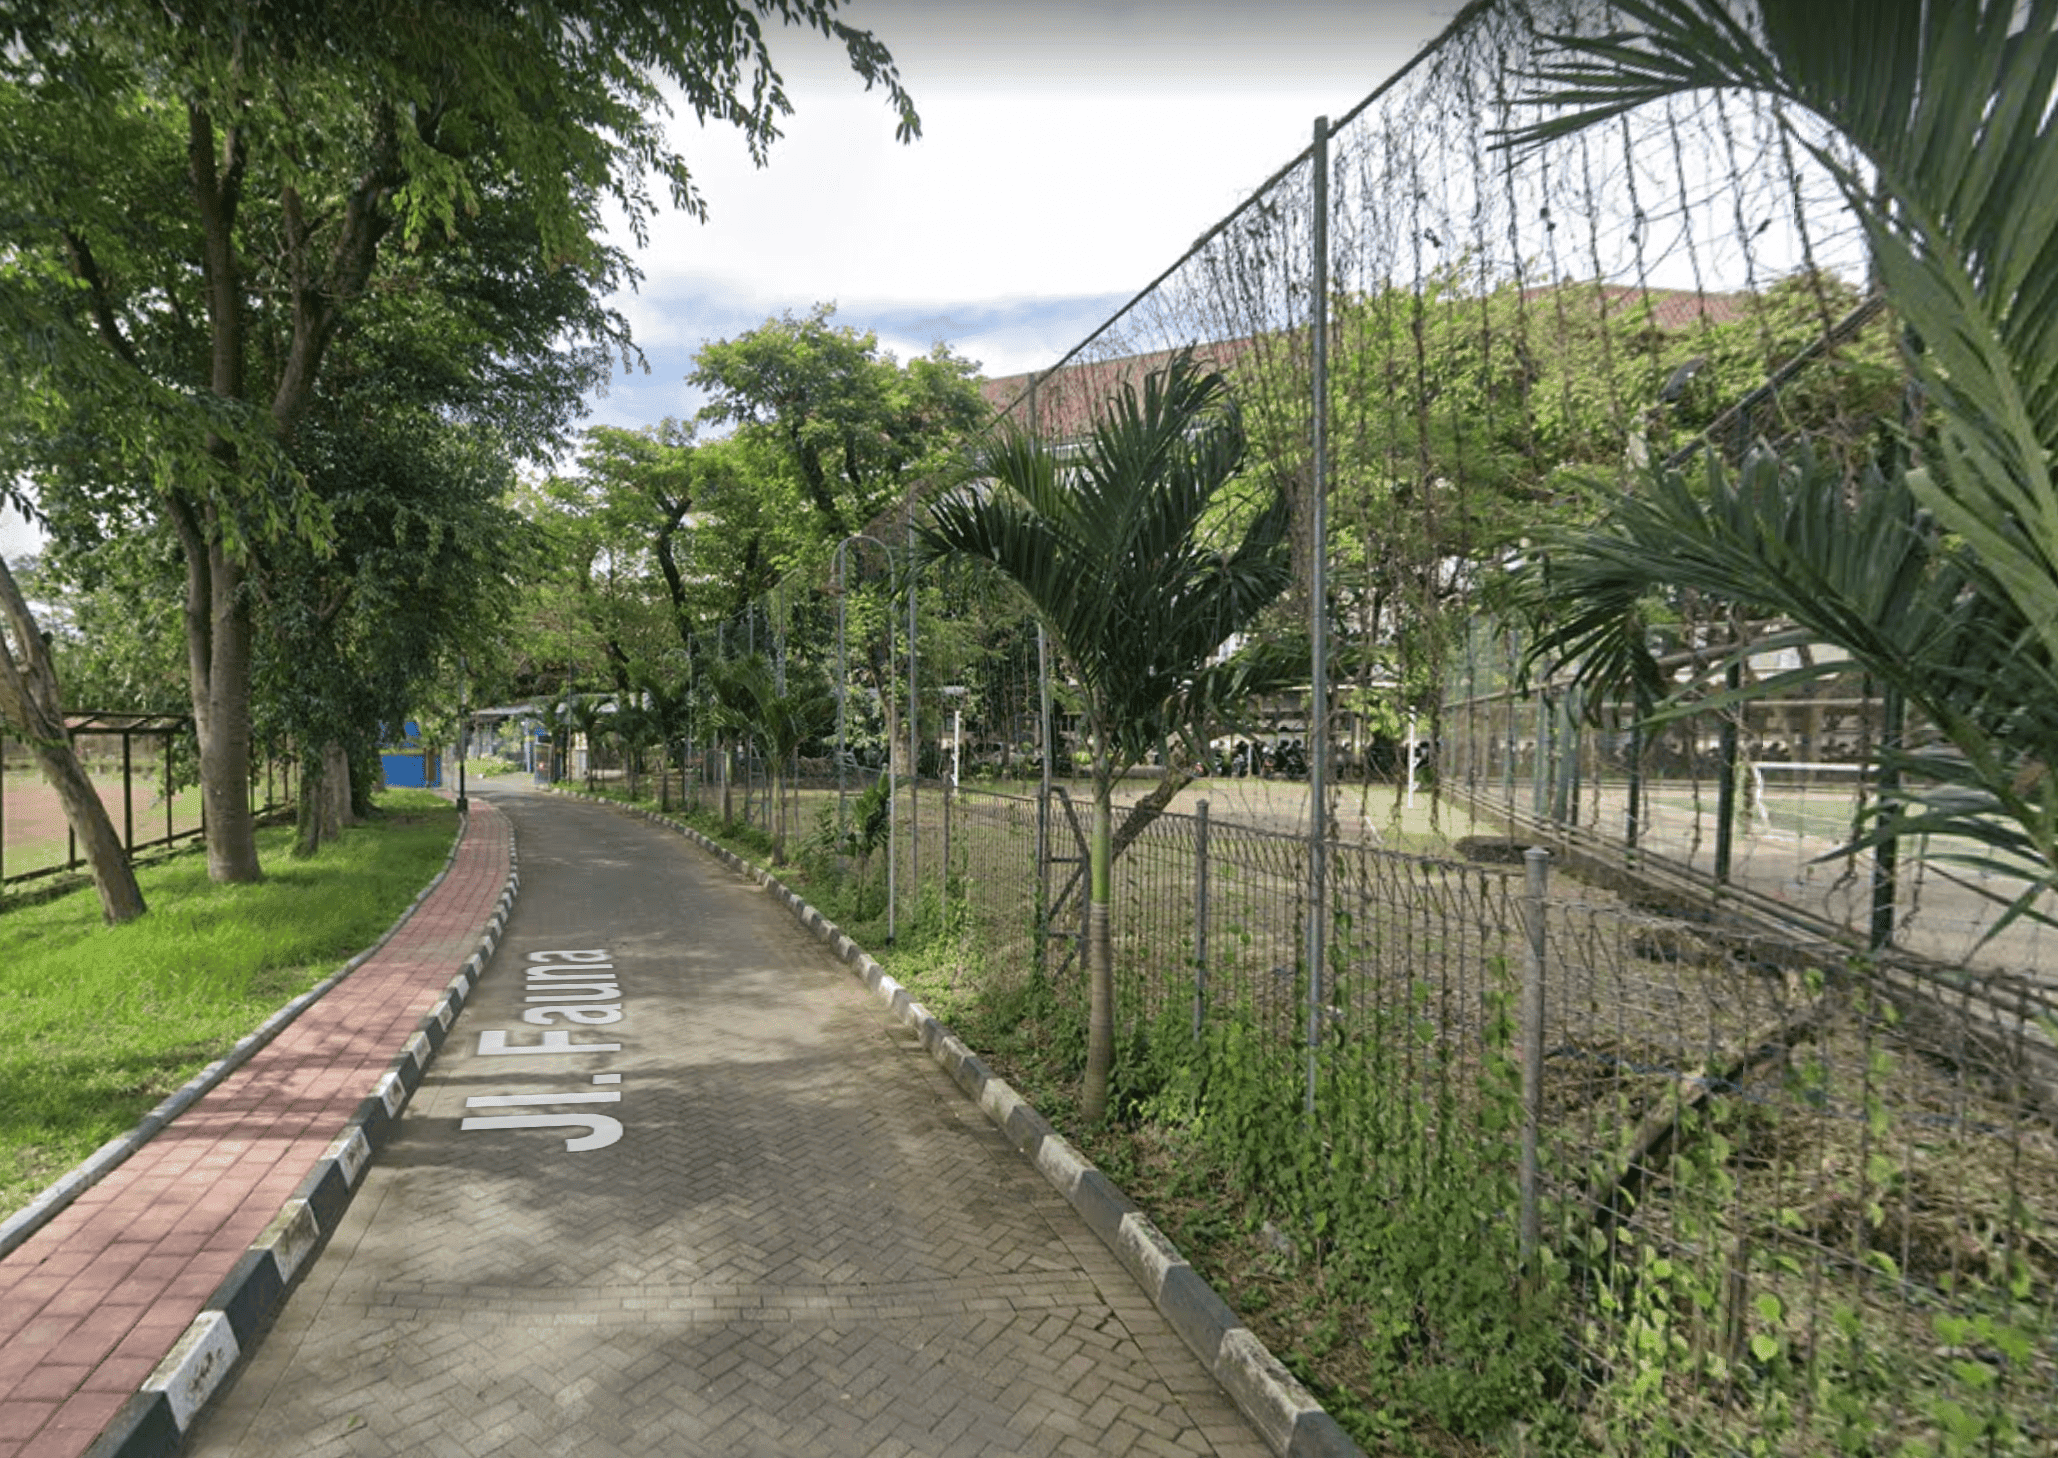
\includegraphics[width=10cm]{contents/chapter-4/pengujian-bergerak/lp-streetview.png}
	\caption{Keadaan di Sekitar Bulaksumur Residence}
	\label{Fig: lp-streetview}
\end{figure}

Visibilitas satelit di setiap titik ditunjukan oleh Gambar \ref{Fig: moving-sats}. Semakin banyak satelit yang digunakan maka warna pada poin akan semakin mendekati warna hijau. Visibilitas satelit terbaik didapat ketika berada di lingkungan Fakultas Teknik, Grha Sabha Pramana, dan Bundaran Universitas Gadjah Mada. Tiga lokasi tersebut memiliki penghalang yang lebih sedikit jika dibandingkan dengan lokasi-lokasi lainnya.

Lokasi dengan visibilitas satelit paling buruk adalah Stadion Pancasila dan Bulaksumur Residence. Gambar \ref{Fig: moving-dop} menunjukan bahwa daerah tersebut juga memiliki nilai DOP paling buruk yang ditandai oleh poin berwarna merah. Terlihat bahwa visibilitas satelit dapat mempengaruhi nilai DOP. 

Visibilitas satelit tidak memberikan peningkatan kualitas \textit{fix} yang signifikan ketika jumlah satelit yang digunakan setidaknya lebih dari lima buah satelit. Jika meninjau visibilitas satelit di sekitar RSUP Dr Sardjito, terlihat bahwa visibilitas satelit tidak sebaik di lingkungan Fakultas Teknik, tetapi nilai DOP tetap berada dalam rentang yang cukup baik.

\begin{figure}[H]
	\centering
	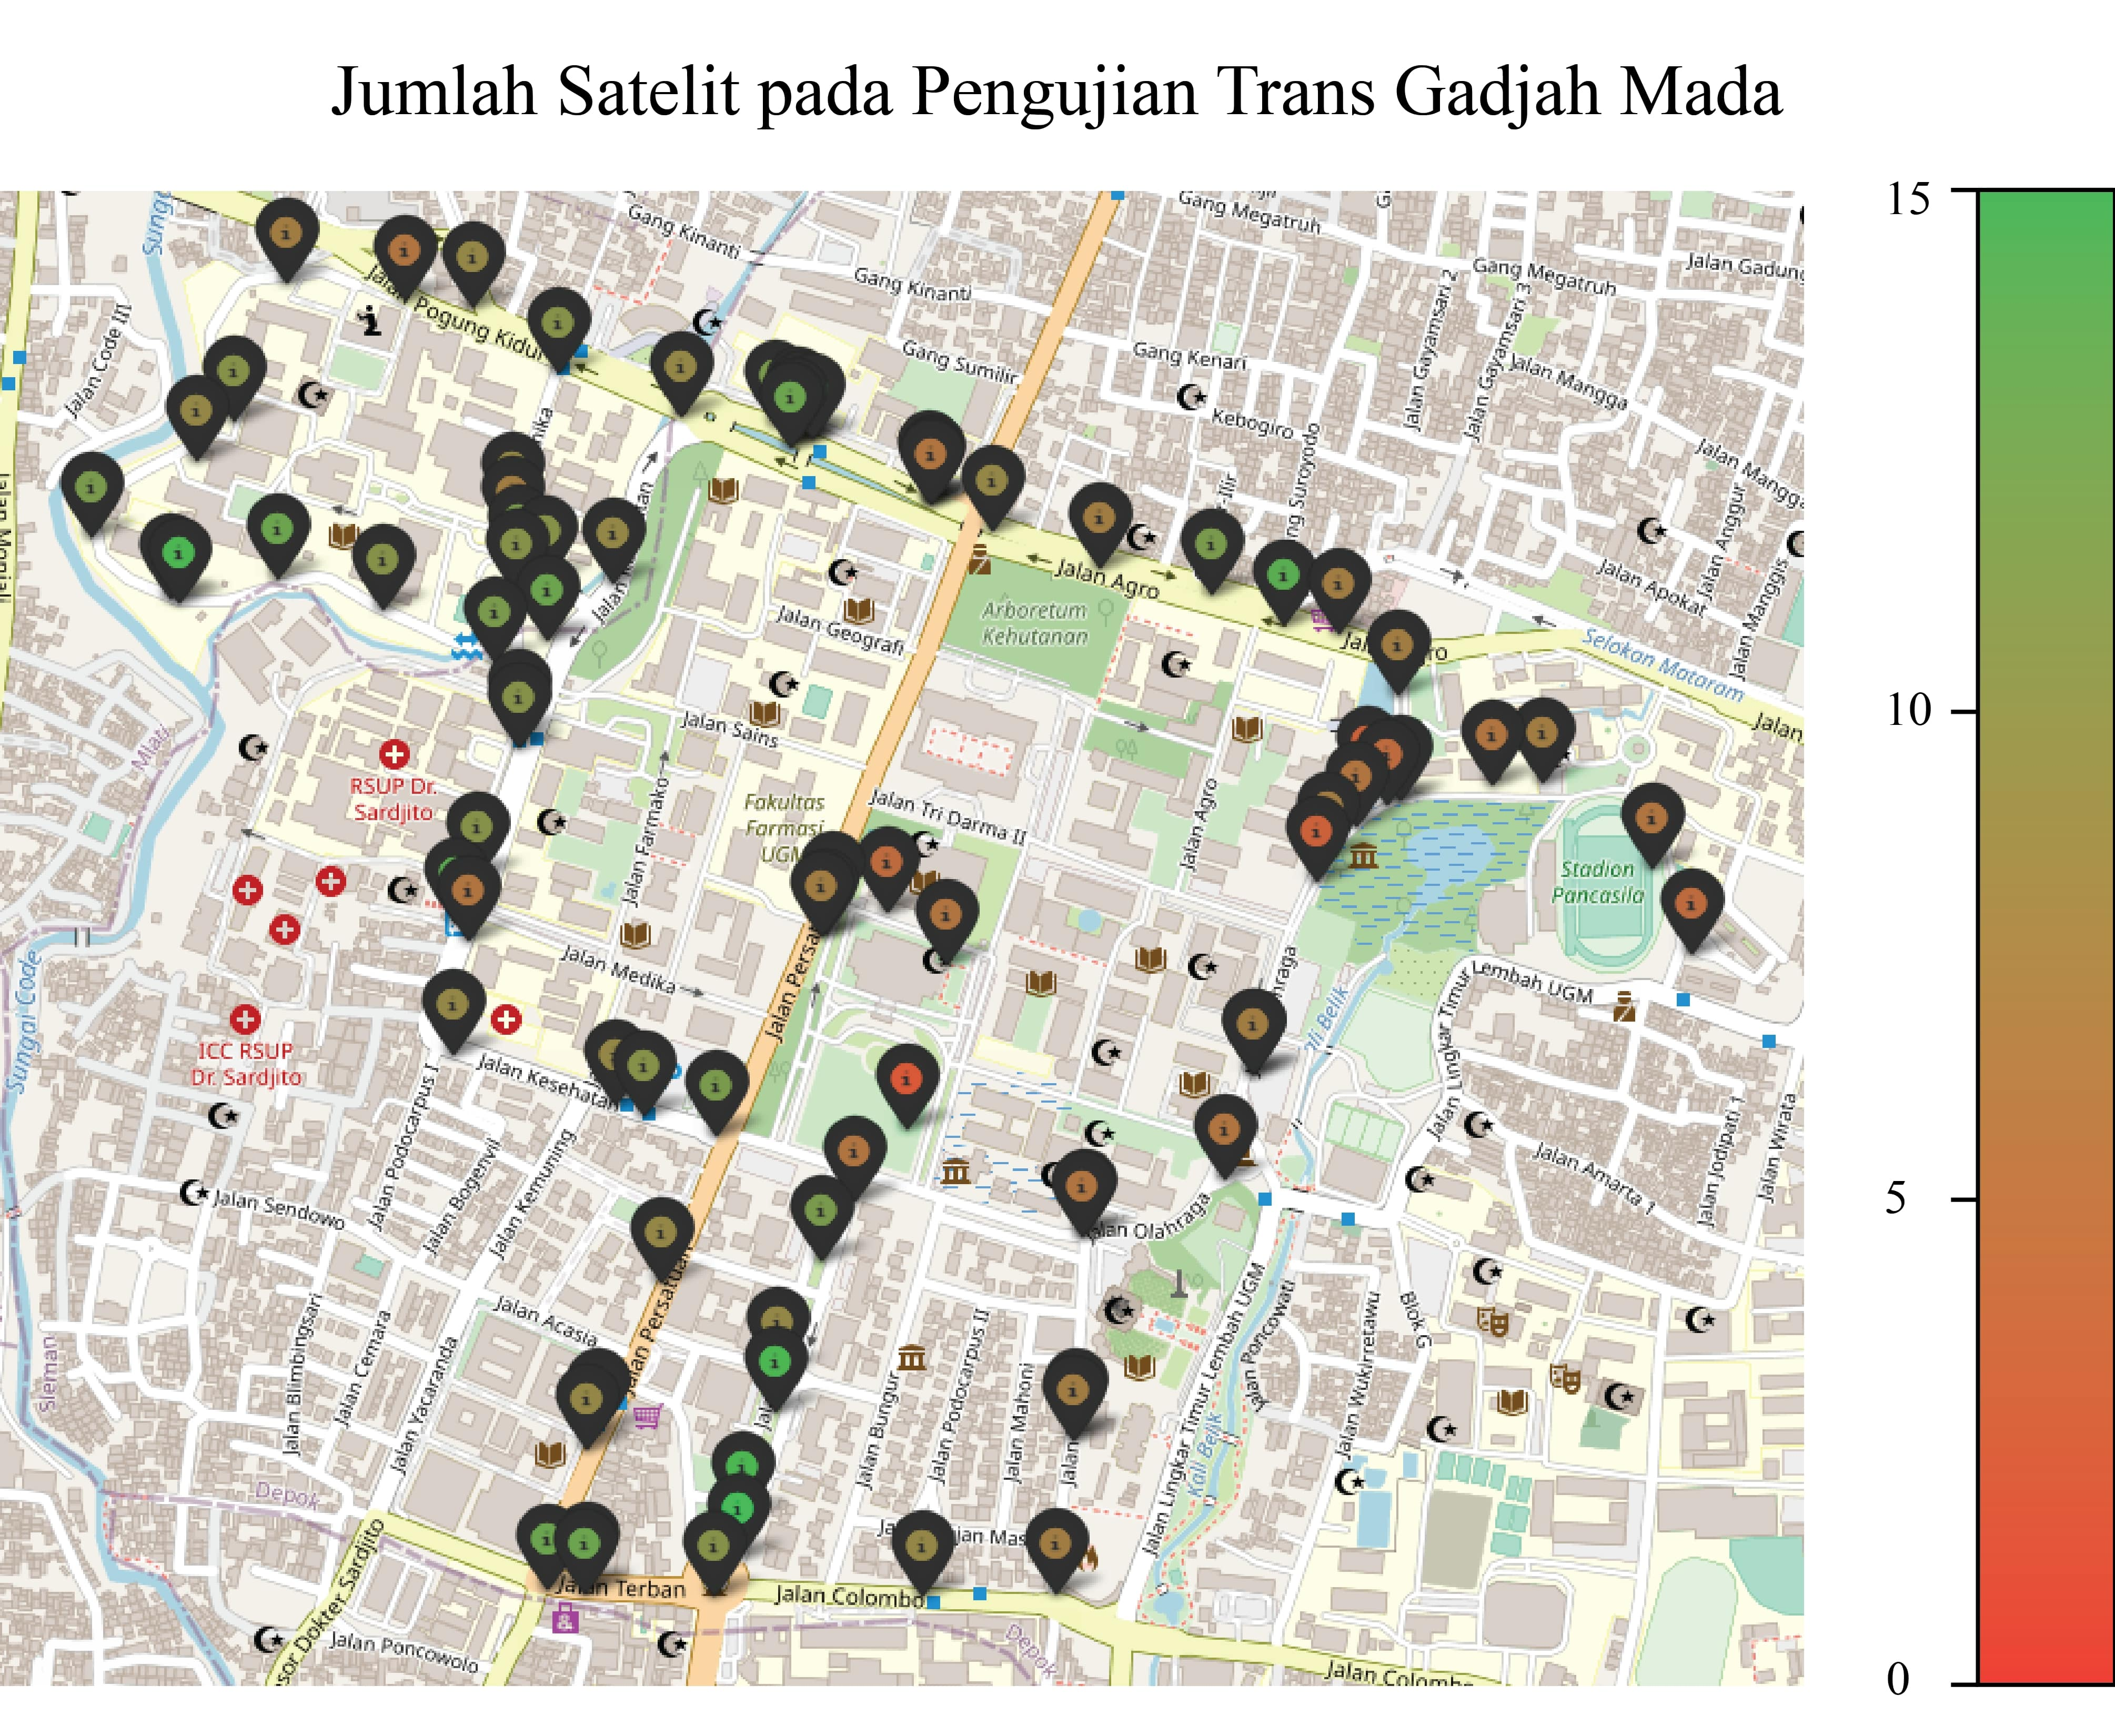
\includegraphics[width=12cm]{contents/chapter-4/pengujian-bergerak/moving-sats.jpg}
	\caption{Pengujian Skenario Dalam Ruangan}
	\label{Fig: moving-sats}
\end{figure}

Hasil pengukuran posisi dengan modul Teseo-LIV3FL sudah merepresentasikan rute sebenarnya yang ditunjukan oleh Gambar \ref{Fig: peta-1b}. Penurunan visibilitas satelit dan kualitas \textit{fix} di beberapa titik tidak berpengaruh signifikan pada hasil akhir secara keseluruhan.